
\chapter{Resultados}
\label{cha:resultados}

\begin{FraseCelebre}
  \begin{Frase}
    Cuando algo es lo suficientemente importante, lo haces incluso si las probabilidades no están a tu favor.
  \end{Frase}
  \begin{Fuente}
    Elon Musk
  \end{Fuente}
\end{FraseCelebre}

\section{Introducción}
\label{sec:intro-resultados}

Este capítulo pretende recoger los resultados obtenidos en la aplicación de los algoritmos empleados y diseñados. Para evaluarlos es necesario disponer de evaluaciones cuantitativas para validar su funcionamiento. En la detección de objetos, los investigadores evalúan sus algoritmos sobre los mismas datasets para poder contrastar resultados con las propuestas de otros investigadores. En la evaluación de los datasets se deben de medir métricas de calidad con lo que se pueda cuantificar el funcionamiento de los algoritmos. En las siguientes secciones se va a especificar los datasets utilizadas y se contemplará el funcionamiento de los algoritmos sobre las mismas.

\section{Entorno experimental}
\label{sec:desarrollo-resultados}

Sabiendo que se va a emplear YOLOv4 en la detección y seguimiento de personas y objetos de interés, en esta sección se va a contemplar los datasets empleadas para ratificar su funcionamiento, las métricas de calidad principales para evaluar el dataset de referencia que se vaya a emplear en el entrenamiento de la red neuronal y por último se va a evaluar el funcionamiento del algoritmo de detección, seguimiento y detección de objetos abandonados sobre los datasets.

\subsection{Datasets utilizados}
\label{subsec:datasets-utilizados}

Se van a describir los datasets más relevantes en la detección de objetos abandonados en los sistemas de videovigilancia así como los datasets de referencia sobre las que se validará previamente en base a las métricas de calidad el modelo entrenado o pre-entrenado utilizado.

En la tabla \ref{tab:datasets} se resumen los contenidos más relevantes de los datasets como son: número de secuencias, longitud media en minutos.

Por otro lado se exponen diferentes \textit{challenges} que se consideran de interés para la detección de objetos abandonados:

\begin{itemize}
    \item I = cambios de iluminación/sombras
    \item R = objetos alejados o pequeños
    \item P = personas estáticas en un punto durante un período de tiempo
    \item O = oclusiones
    \item LR = resolución vídeo baja
    \item RO = objetos abandonados o eliminados
\end{itemize}

\begin{table}[ht]
\centering
\caption{Datasets utilizados en la evaluación de los algoritmos}
\label{tab:datasets}
\begin{tabular}{lcccc}
\hline
\textbf{Nombre del dataset} & \textbf{\# Secuencias} & \textbf{\begin{tabular}[c]{@{}c@{}}Longitud media\\ (min)\end{tabular}} & \textbf{Escenario} & \textbf{Challenge} \\ \hline
ABODA                       & 11                     & 1,90                                                                    & Interior/exterior  & I, R, P, O         \\
AVSSAB2007                  & 3                      & 3,46                                                                    & Estación de metro  & I, R, P, O         \\
PETS2007                    & 28                     & 1,96                                                                    & Aeropuerto         & I, R, P, O         \\
GBA2018                     & 8                      & 0,74                                                                    & Interior           & I, R, P, O, RO     \\ \hline
\end{tabular}
\end{table}
\aviso{Una página por cada dataset!!!}

\newpage

\subsubsection{PETS 2007 Dataset}

\begin{figure}[ht]
  \centering
  \begin{subfigure}[b]{0.4\textwidth}
    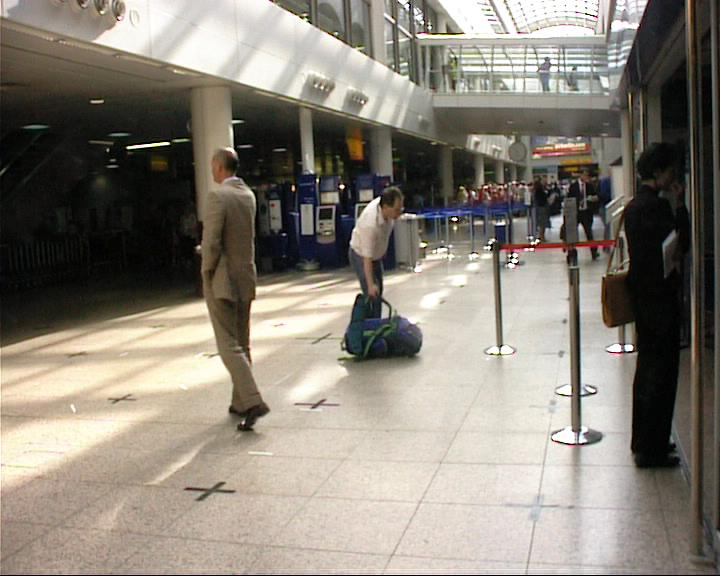
\includegraphics[width=\textwidth]{img/chapters/resultados/datasets/pets2007_1.jpg}
    \caption{}
    \label{fig:pets2007_1}
  \end{subfigure}
  \qquad\qquad
  \begin{subfigure}[b]{0.4\textwidth}
    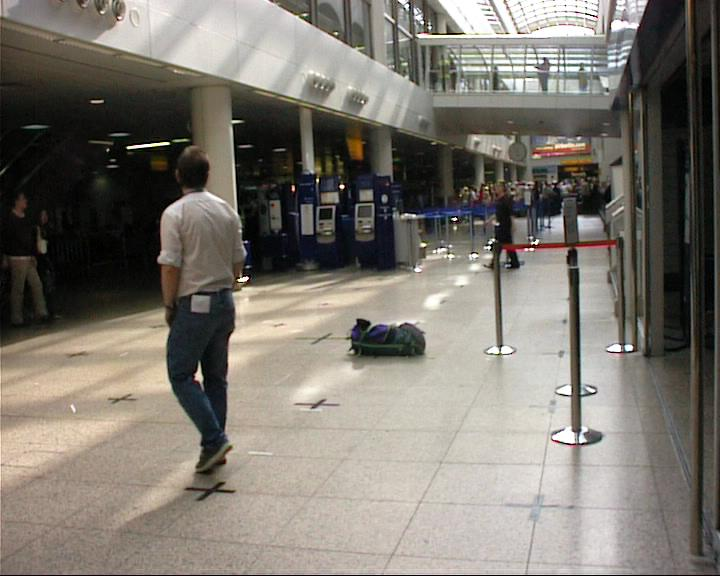
\includegraphics[width=\textwidth]{img/chapters/resultados/datasets/pets2007_2.jpg}
    \caption{}
    \label{fig:pets2007_2}
  \end{subfigure}
  \caption{Imágenes extraídas del dataset PETS2007 \cite{pets2007-dataset}.
    (\protect\subref{fig:pets2007_1}) Frame donde un hombre deja su equipaje en el suelo.
    (\protect\subref{fig:pets2007_2}) Otro frame donde el abandona el lugar sin su equipaje.}
  \label{fig:pets2007_S08}
\end{figure}

\begin{figure}[ht]
  \centering
  \begin{subfigure}[b]{0.4\textwidth}
    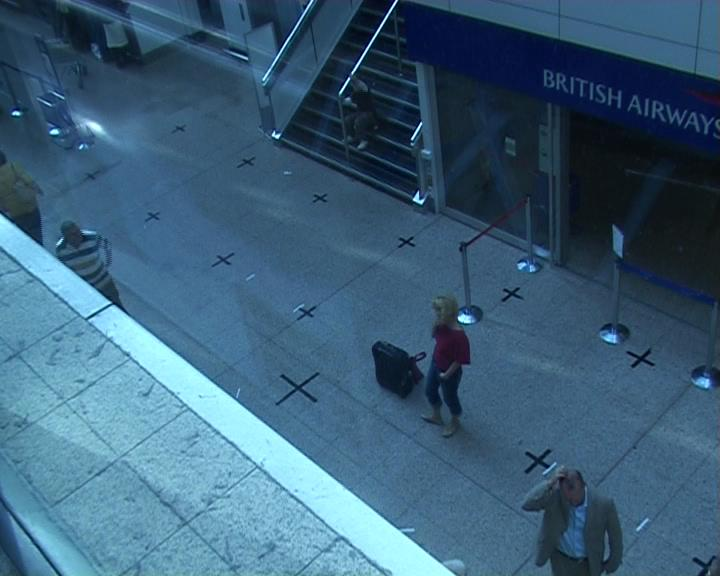
\includegraphics[width=\textwidth]{img/chapters/resultados/datasets/pets2007_3.jpg}
    \caption{}
    \label{fig:pets2007_3}
  \end{subfigure}
  \qquad\qquad
  \begin{subfigure}[b]{0.4\textwidth}
    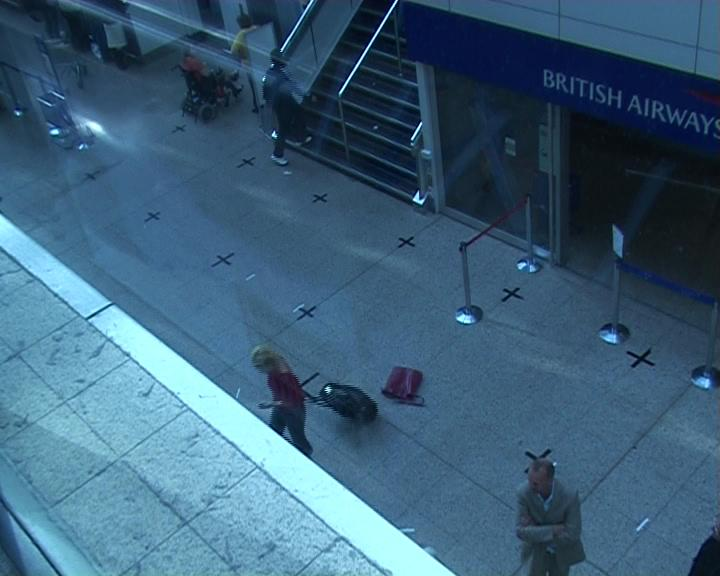
\includegraphics[width=\textwidth]{img/chapters/resultados/datasets/pets2007_4.jpg}
    \caption{}
    \label{fig:pets2007_4}
  \end{subfigure}
  \caption{Imágenes extraídas del dataset PETS2007 \cite{pets2007-dataset}.
    (\protect\subref{fig:pets2007_3}) Frame donde una mujer se encuentra junto a su equipaje.
    (\protect\subref{fig:pets2007_4}) Otro frame donde la mujer abandona el lugar sin su bolso.}
  \label{fig:pets2007_S07}
\end{figure}

\newpage

\subsubsection{AVSS AB 2007 Dataset}

Se ha utilizado las secuencias dedicadas a la detección de objetos abandonados del dataset \gls{avss}. Una persona ha colocado un objeto que es de su pertenencia sobre el andén. La persona abandona el área de detección sin el objeto durante más de 60 segundos. Durante ese tiempo el objeto permanece estático en el área de detección. Este dataset está formado por tres secuencias de vídeo grabadas a una resolución de 720 x 576 píxeles a 25 \gls{fps}. En modelo de la cámara no se especifica.

La región de interés está divida en tres zonas: cercana, media, lejos. En cada una de las secuencias de vídeo el objeto que es abandonado se encuentra en cada una de estas zonas.

\begin{figure}[ht]
  \centering
  \begin{subfigure}[b]{0.4\textwidth}
    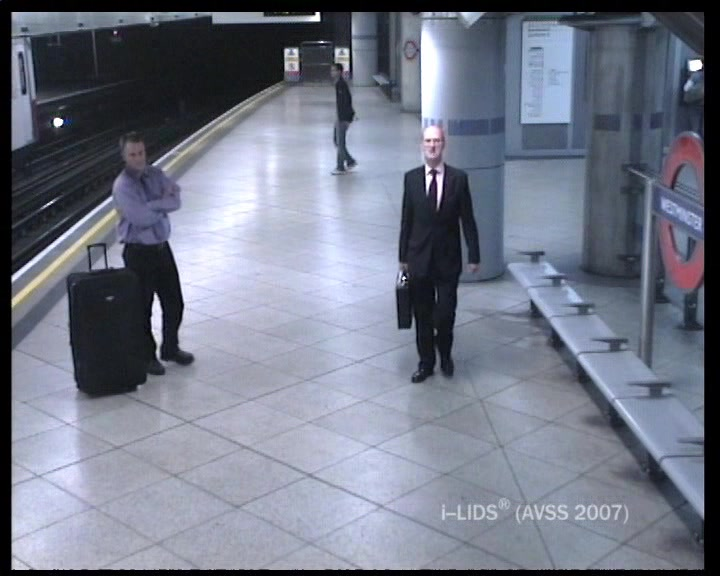
\includegraphics[width=\textwidth]{img/chapters/resultados/datasets/AVSSAB_1.jpg}
    \caption{}
    \label{fig:avssab2007_1}
  \end{subfigure}
  \qquad\qquad
  \begin{subfigure}[b]{0.4\textwidth}
    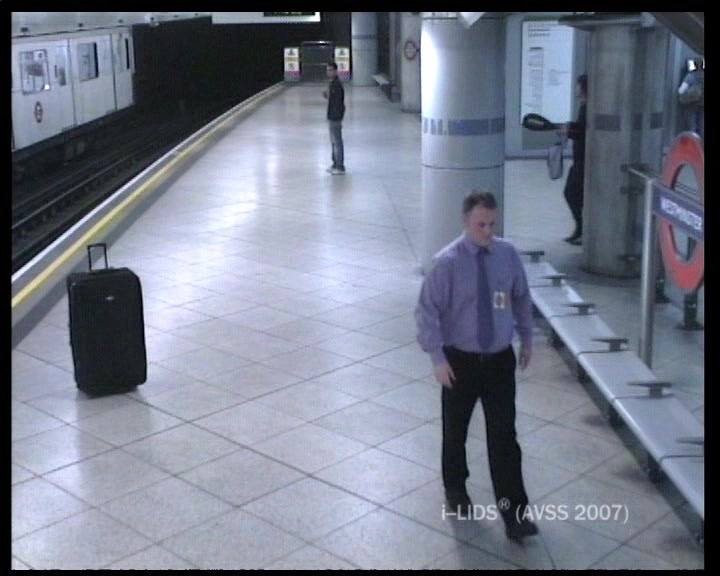
\includegraphics[width=\textwidth]{img/chapters/resultados/datasets/AVSSAB_2.jpg}
    \caption{}
    \label{fig:avssab2007_2}
  \end{subfigure}
  \caption{Imágenes extraídas del dataset AVSS AB 2007 \cite{AVSSAB2007-dataset}.
    (\protect\subref{fig:avssab2007_1}) Frame donde un hombre se encuentra junto a su maleta en la zona cercana del andén del metro.
    (\protect\subref{fig:avssab2007_2}) Otro frame donde donde el hombre abandona la zona cercana su maleta durante más de 60 segundos.}
  \label{fig:avssab2007_easy}
\end{figure}

\begin{figure}[ht]
  \centering
  \begin{subfigure}[b]{0.4\textwidth}
    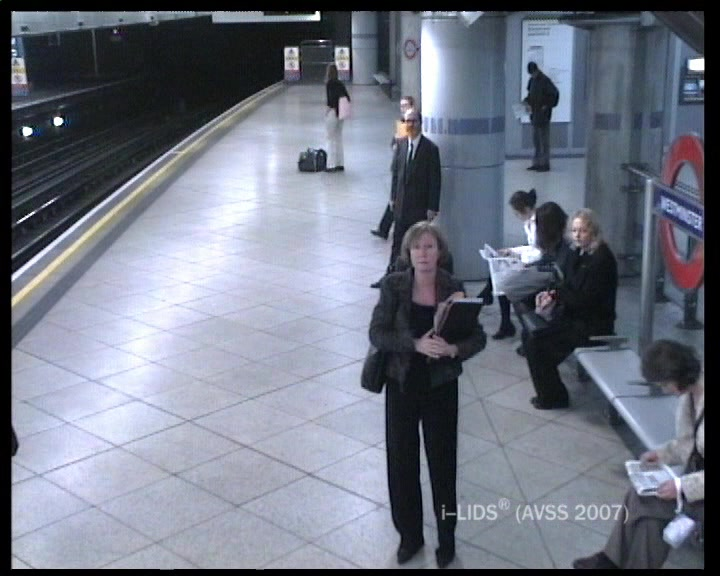
\includegraphics[width=\textwidth]{img/chapters/resultados/datasets/AVSSAB_3.jpg}
    \caption{}
    \label{fig:avssab2007_3}
  \end{subfigure}
  \qquad\qquad
  \begin{subfigure}[b]{0.4\textwidth}
    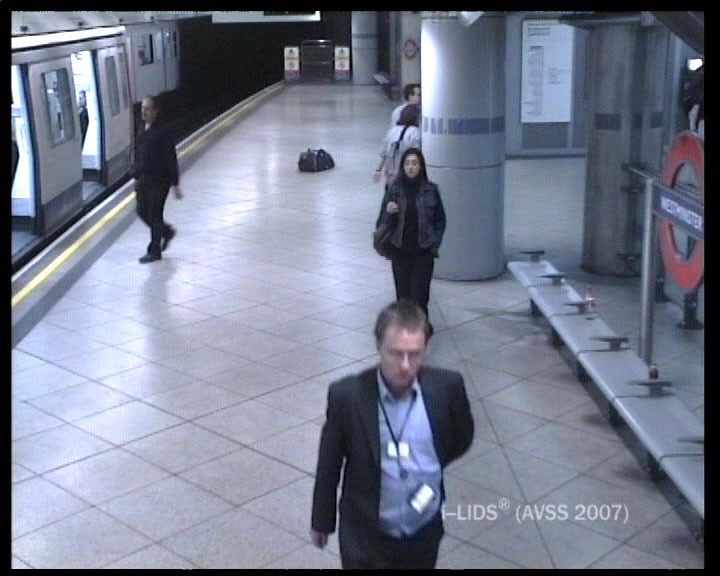
\includegraphics[width=\textwidth]{img/chapters/resultados/datasets/AVSSAB_4.jpg}
    \caption{}
    \label{fig:avssab2007_4}
  \end{subfigure}
  \caption{Imágenes extraídas del dataset AVSS AB 2007 \cite{AVSSAB2007-dataset}.
    (\protect\subref{fig:avssab2007_3}) Frame donde una mujer se encuentra junto a su bolsa de mano en la zona media del andén del metro.
    (\protect\subref{fig:avssab2007_4}) Otro frame donde la bolsa de mano se encuentra abandonada en la zona media del andén del metro.}
  \label{fig:avssab2007_medium}
\end{figure}

\newpage

\subsubsection{GBA 2018 Dataset}

El dataset \gls{gba2018} del grupo de investigación \gls{geintra} fue grabado en la \gls{eps} de la \gls{uah} durante la realización del \gls{tfm} de David Valdivieso López \cite{valdivieso2018}. Está orientado a la evaluación de algoritmos de detección de objetos abandonados. El dataset está formado 8 secuencias en 2 escenarios distintos grabadas con una GoPro HERO4 a una resolución de 1920 x 1080 píxeles a 60 \gls{fps}.

En el primer escenario se muestra como región de interés el Hall de la \gls{eps} desde un plano alejado donde ocurren eventos como abandono de maletas, mochilas y bolsas de mano.

\begin{figure}[ht!]
  \centering
  \begin{subfigure}[b]{0.45\textwidth}
    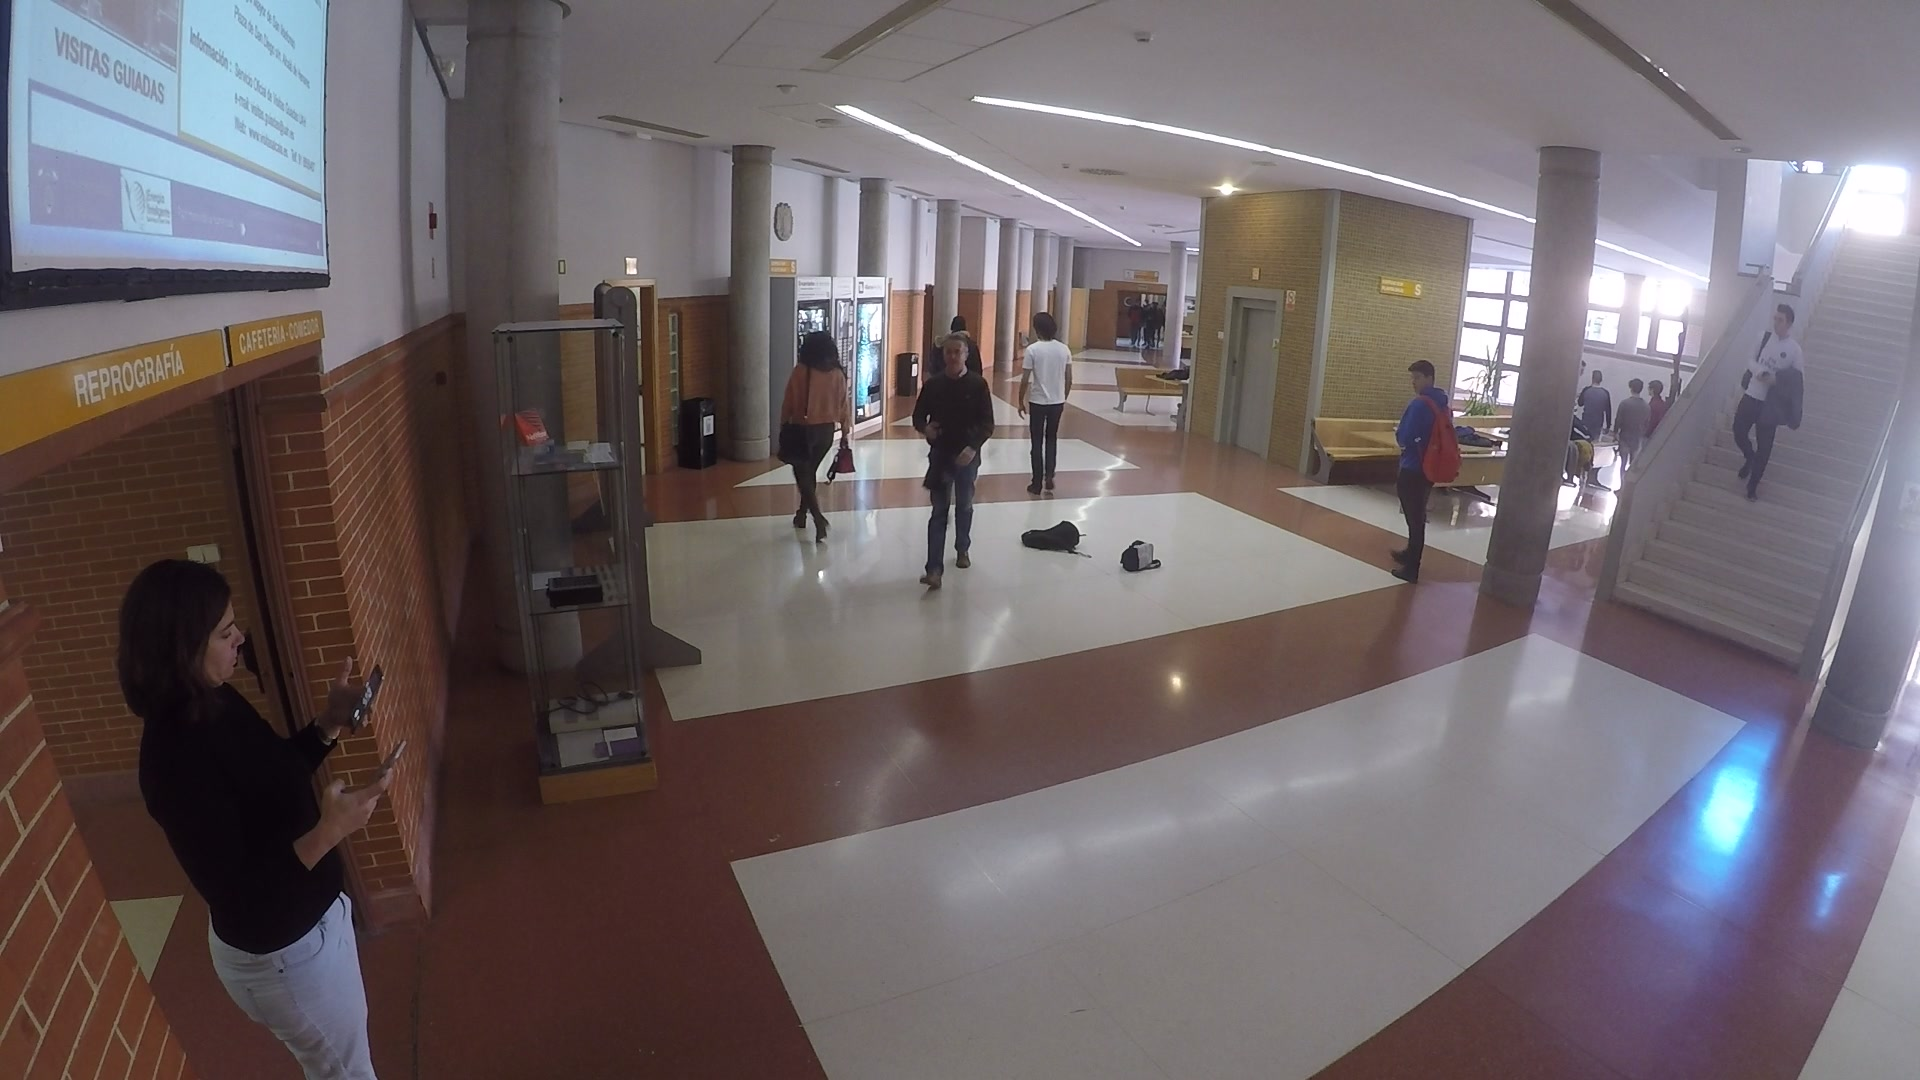
\includegraphics[width=\textwidth]{img/chapters/resultados/datasets/GBA_1.jpg}
    \caption{}
    \label{fig:GBA_1}
  \end{subfigure}
  \qquad\qquad
  \begin{subfigure}[b]{0.45\textwidth}
    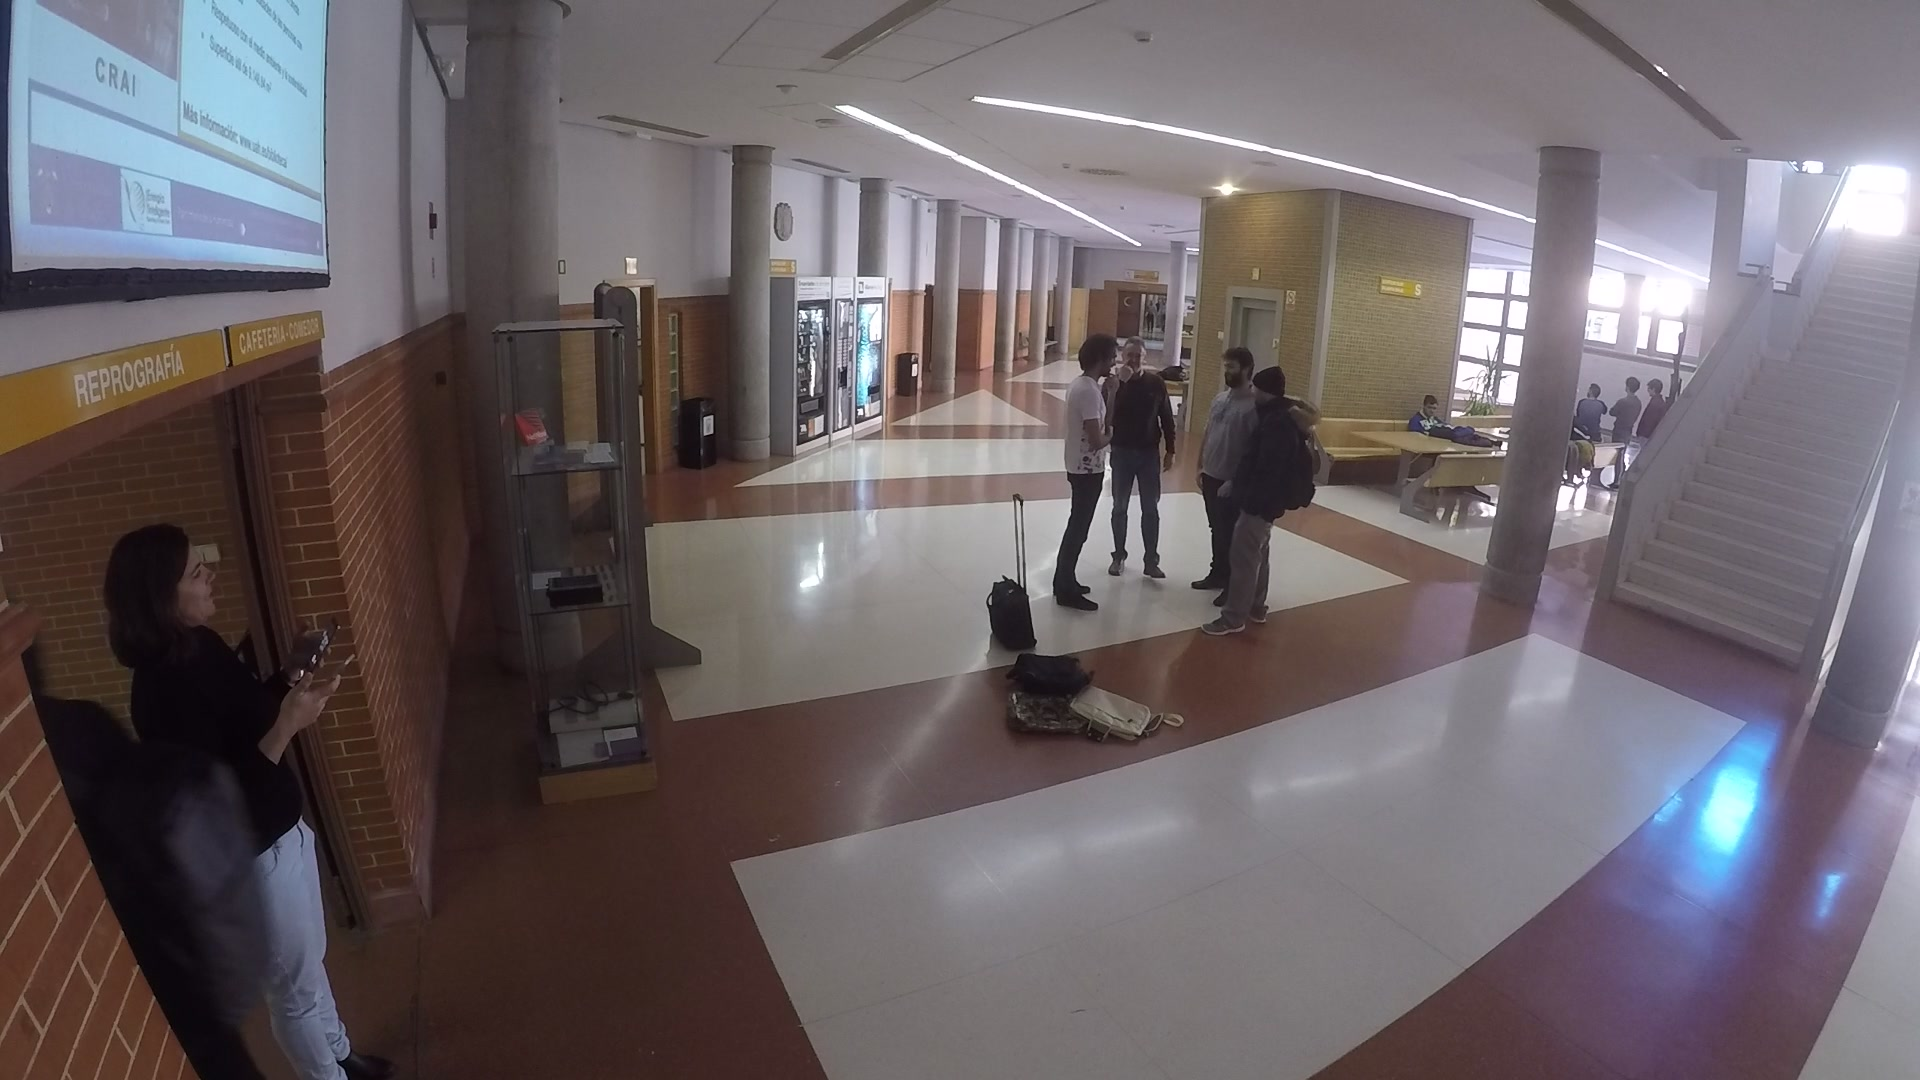
\includegraphics[width=\textwidth]{img/chapters/resultados/datasets/GBA_2.jpg}
    \caption{}
    \label{fig:GBA_2}
  \end{subfigure}
  \caption{Imágenes extraídas de secuencias del primer escenario del dataset GBA 2018 \cite{gba-dataset}.
    (\protect\subref{fig:GBA_1}) Frame donde dos bolsas de mano han sido abandonadas en mitad del hall.
    (\protect\subref{fig:GBA_2}) Otro frame donde varias bolsas y maletas están alejadas de sus propietarios.}
  \label{fig:GBA1}
\end{figure}

La región de interés del segundo escenario se encuentra en el pasillo que conecta el hall con la cafetería. El plano de la grabación es más cercano respecto al primer escenario con lo que se consideran secuencias más fáciles de evaluar ya que no se encuentran elementos de interés alejados.

\begin{figure}[ht!]
  \centering
  \begin{subfigure}[b]{0.45\textwidth}
    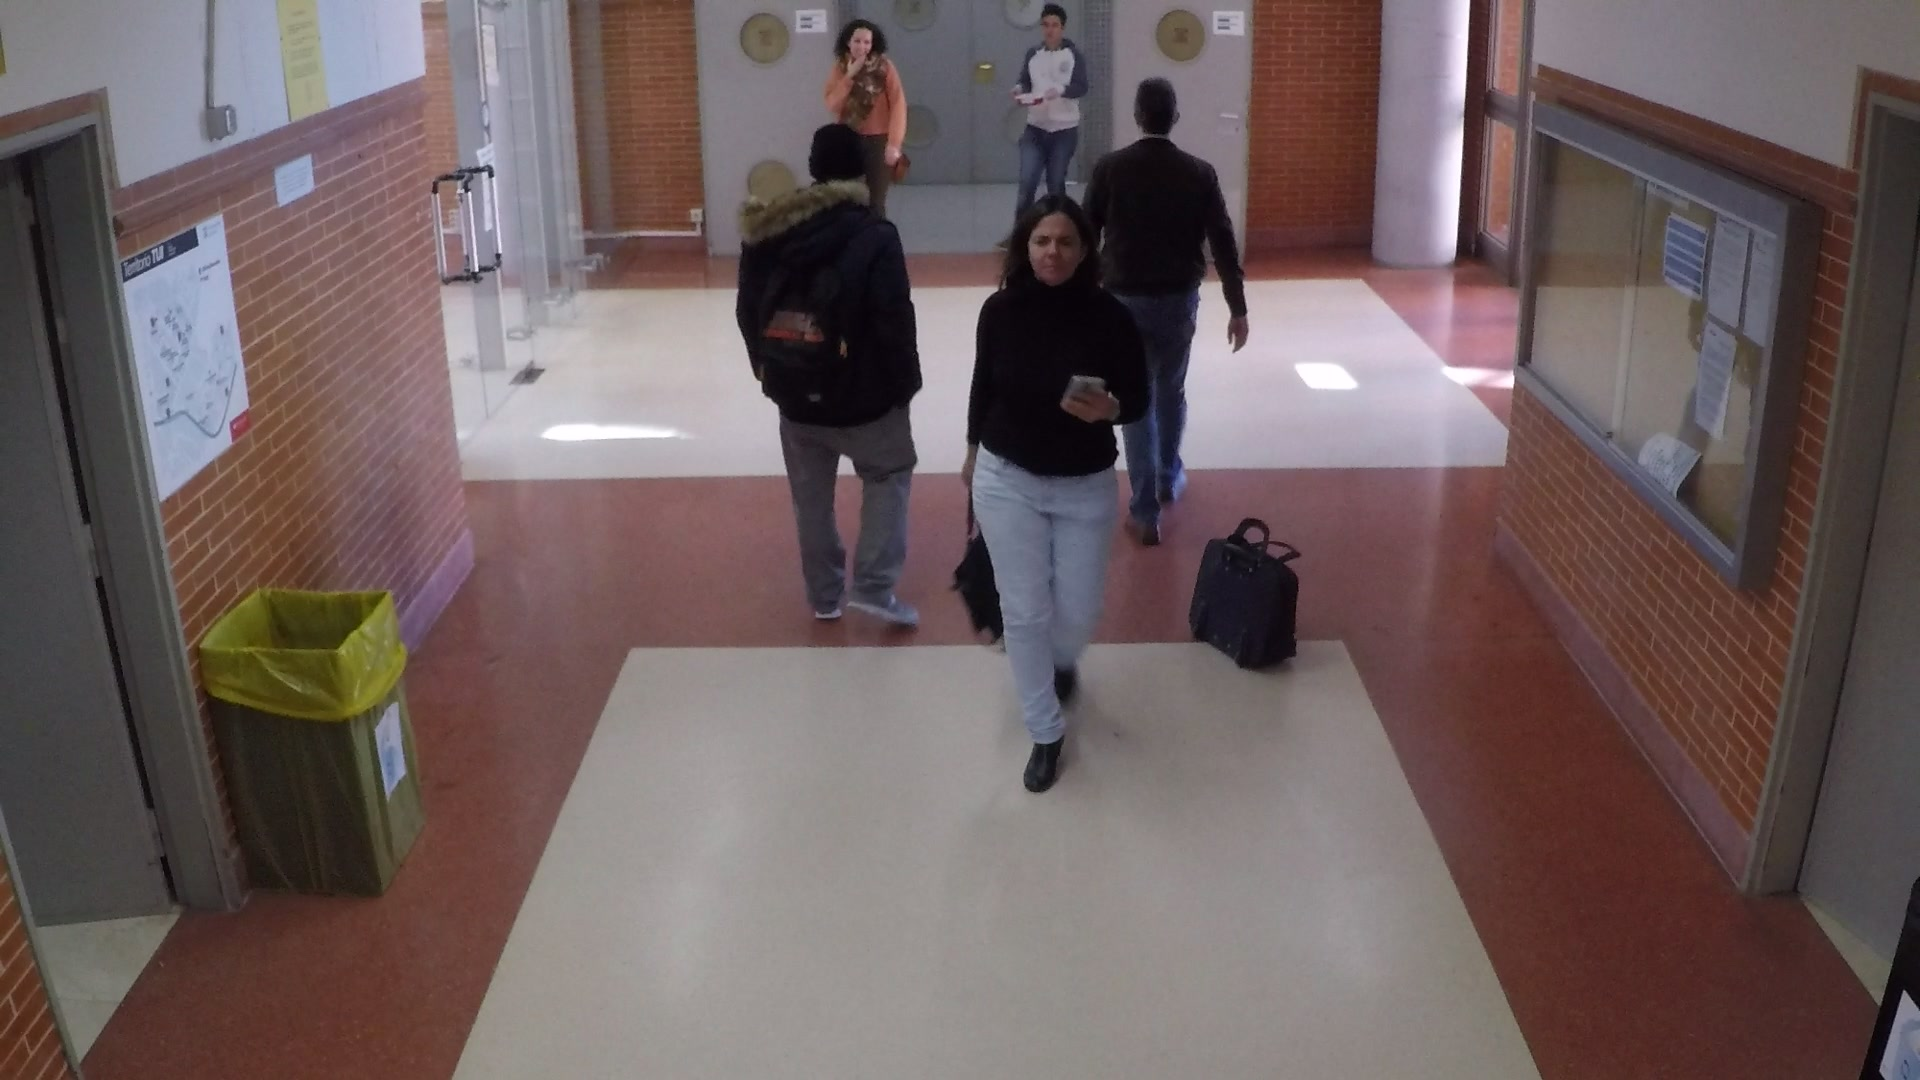
\includegraphics[width=\textwidth]{img/chapters/resultados/datasets/GBA_3.jpg}
    \caption{}
    \label{fig:GBA_3}
  \end{subfigure}
  \qquad\qquad
  \begin{subfigure}[b]{0.45\textwidth}
    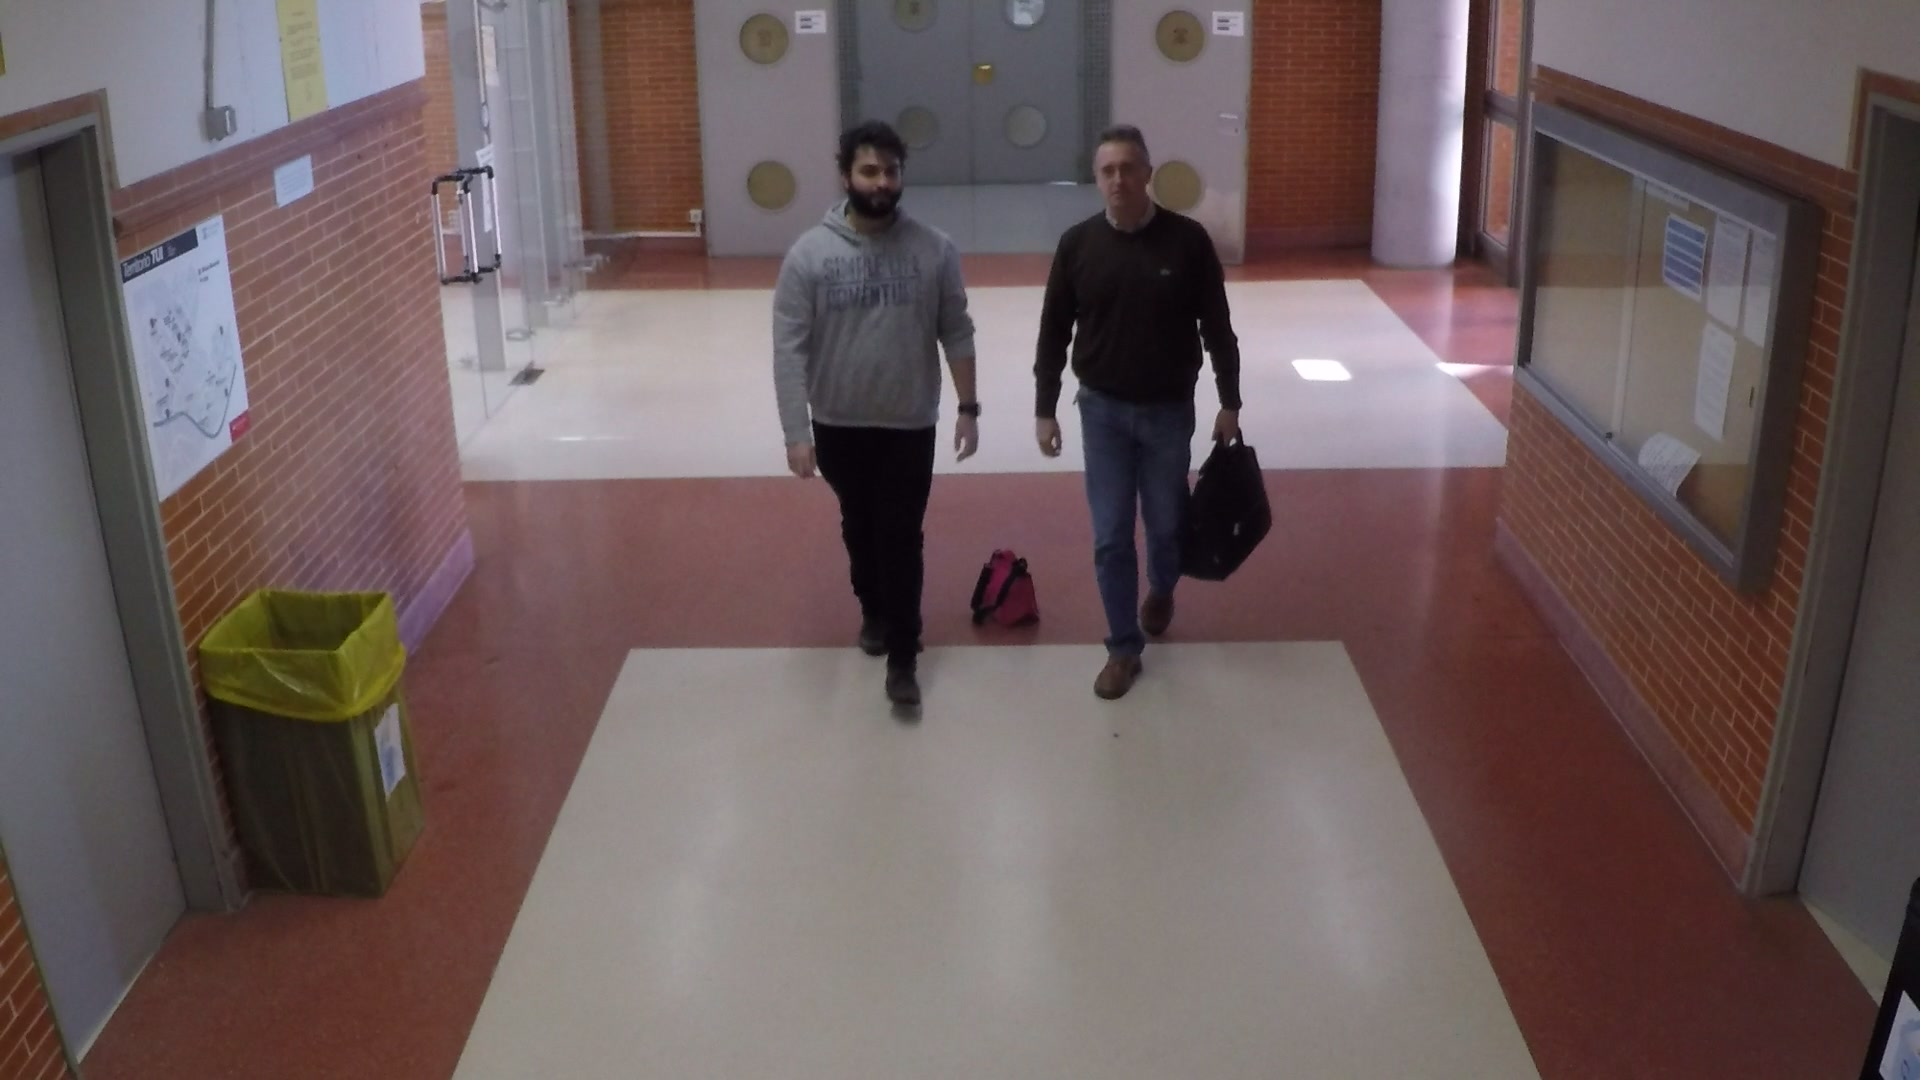
\includegraphics[width=\textwidth]{img/chapters/resultados/datasets/GBA_4.jpg}
    \caption{}
    \label{fig:GBA_4}
  \end{subfigure}
  \caption{Imágenes extraídas de secuencias del segundo escenario del dataset GBA 2018 \cite{gba-dataset}.
    (\protect\subref{fig:GBA_3}) Frame donde una bolsa de mano es abandonada en el pasillo de la cafetería.
    (\protect\subref{fig:GBA_4}) Otro frame donde dos personas abandonan una pequeña bolsa de mano.}
  \label{fig:GBA2}
\end{figure}

\newpage

\subsubsection{ABODA Dataset}

El dataset \gls{aboda} está dedicado a la detección de objetos abandonados en escenarios muy diferenciados.

\begin{figure}[ht]
  \centering
  \begin{subfigure}[b]{0.4\textwidth}
    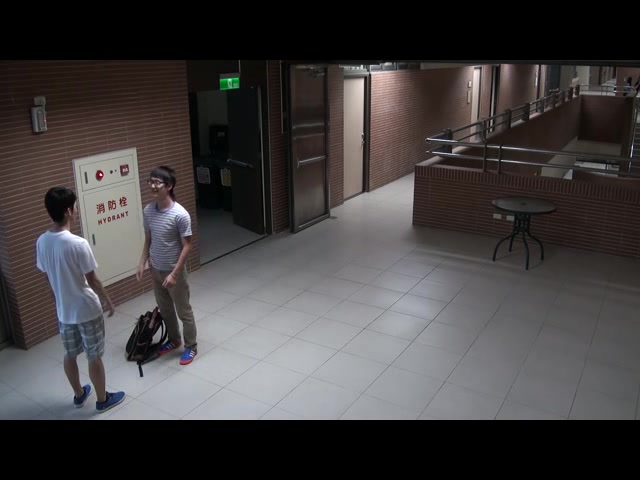
\includegraphics[width=\textwidth]{img/chapters/resultados/datasets/aboda_1.jpg}
    \caption{}
    \label{fig:aboda_1}
  \end{subfigure}
  \qquad\qquad
  \begin{subfigure}[b]{0.4\textwidth}
    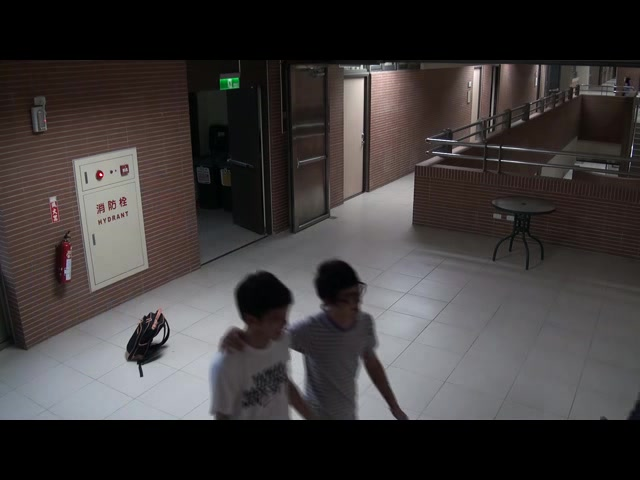
\includegraphics[width=\textwidth]{img/chapters/resultados/datasets/aboda_2.jpg}
    \caption{}
    \label{fig:aboda_2}
  \end{subfigure}
  \caption{Imágenes extraídas del dataset ABODA \cite{aboda-dataset}.
    (\protect\subref{fig:aboda_1}) Frame donde dos chicos conversan en el hall.
    (\protect\subref{fig:aboda_2}) Otro frame donde los dos chicos abandonan una mochila.}
  \label{fig:aboda1}
\end{figure}

\begin{figure}[ht]
  \centering
  \begin{subfigure}[b]{0.4\textwidth}
    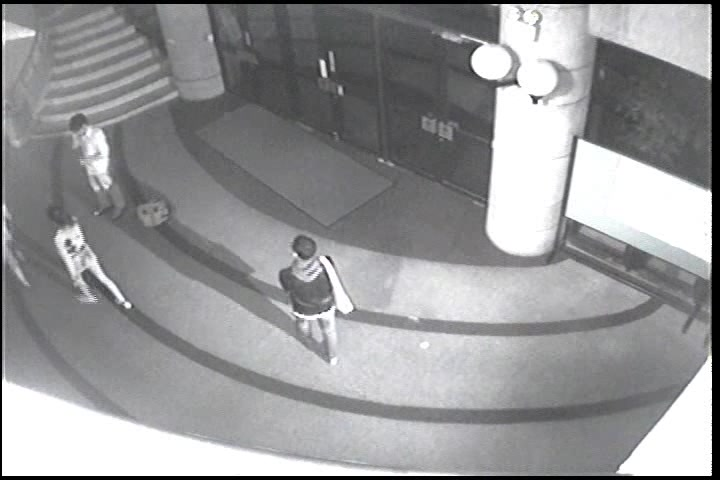
\includegraphics[width=\textwidth]{img/chapters/resultados/datasets/aboda_3.jpg}
    \caption{}
    \label{fig:aboda_3}
  \end{subfigure}
  \qquad\qquad
  \begin{subfigure}[b]{0.4\textwidth}
    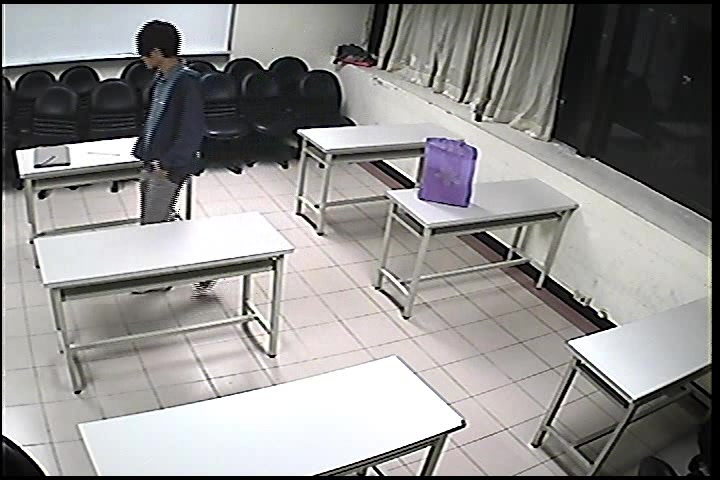
\includegraphics[width=\textwidth]{img/chapters/resultados/datasets/aboda_4.jpg}
    \caption{}
    \label{fig:aboda_4}
  \end{subfigure}
  \caption{Imágenes extraídas del dataset ABODA \cite{aboda-dataset}.
    (\protect\subref{fig:aboda_3}) Frame donde un individuo entra a un aula con una bolsa de mano.
    (\protect\subref{fig:aboda_4}) Otro frame donde el individuo abandona la bolsa en la mesa.}
  \label{fig:aboda2}
\end{figure}

\newpage

\subsubsection{MS COCO 2017 Dataset}
\label{subsubsec:coco-dataset}

\textcolor{red}{El dataset MS COCO 2017 es gran datasets que contiene más de 200 000 imágenes distribuidas en 80 clases de objetos que representan escenas del mundo real. Es un dataset lo suficientemente grande para que una red bien entrenada con este dataset sea capaz de aprender características visuales de calidad para el reconocimiento y detección de objetos en imágenes.}

\begin{figure}[ht]
\centering
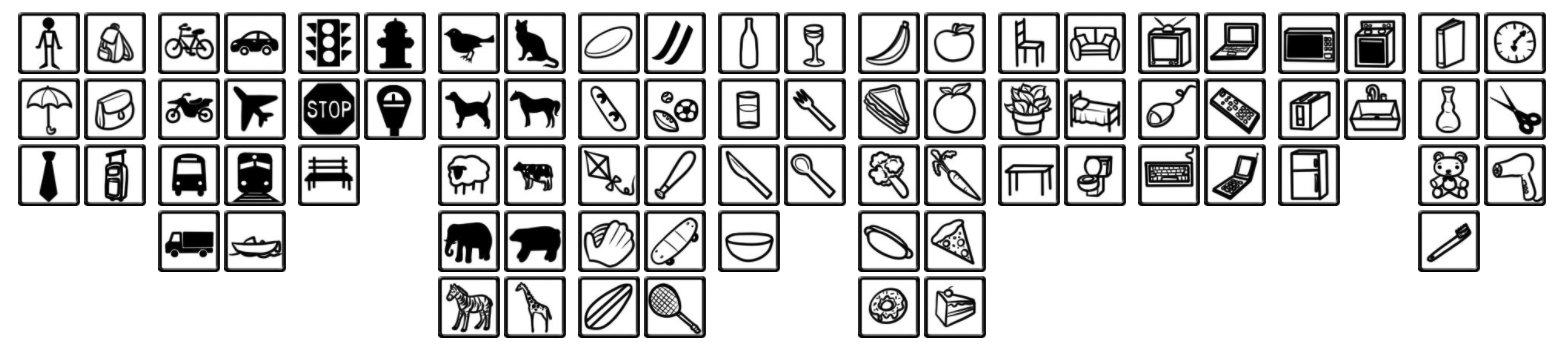
\includegraphics[width=0.9\textwidth]{img/chapters/resultados/datasets/cocodataset.png}
\caption{\label{fig:cocodataset}Categorías de objetos del dataset MS COCO 2017}
\end{figure}

\newpage

\subsubsection{Open Images Dataset v4}
\label{subsubsec:OIDv4-dataset}

\begin{figure}[ht]
\centering
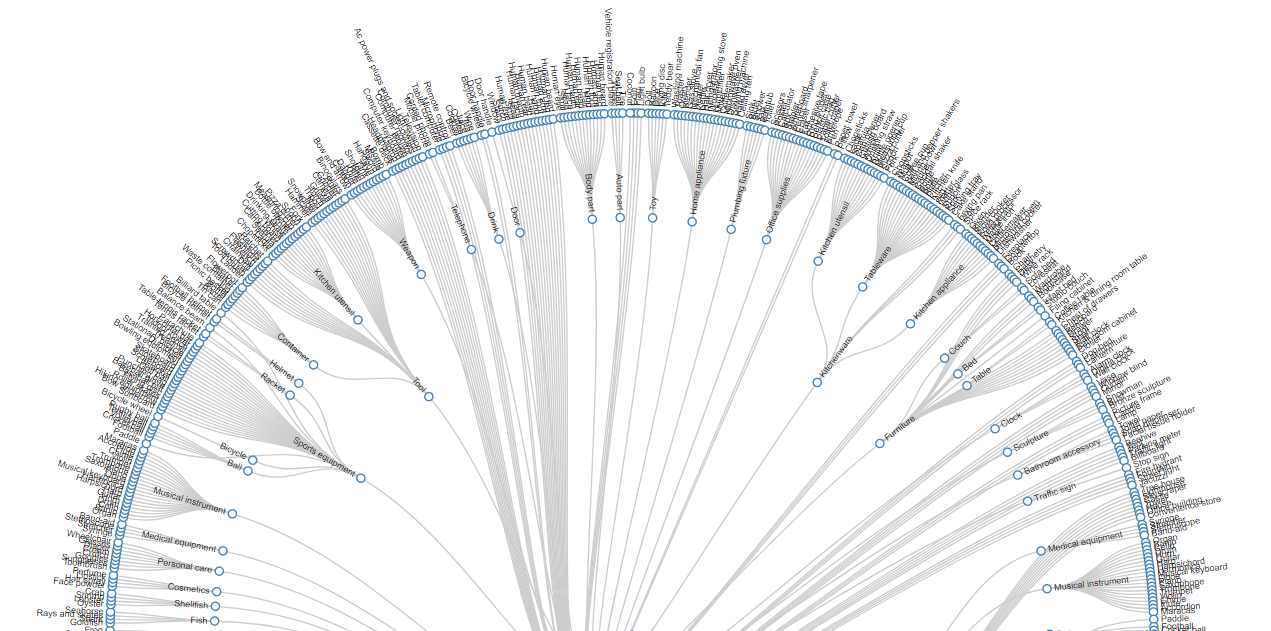
\includegraphics[width=0.7\textwidth]{img/chapters/resultados/datasets/oid-classes.png}
\caption{\label{fig:oiddataset}Categorías de objetos del dataset Open Images Dataset v4}
\end{figure}

\newpage

\subsection{Métricas de calidad}
\label{subsec:metricas-calidad}

\textcolor{red}{Ver TFM de Ana Ruipérez Gómez o Pedro López Miguel para ver como ha redactado las métricas} \pendiente{ojo a esto!!!}

En esta sección se va a exponer las distintas métricas \cite{padillaCITE2020} que han sido utilizadas para evaluar el dataset utilizado para el entrenamiento de la red neuronal.

\subsubsection{Intersección sobre la unión (IoU)}
\label{subsubsec:iou}

\gls{iou} es una medida basada en el índice Jaccard que evalúa la superposición entre dos cuadros delimitadores. Requiere un cuadro delimitador de verdad del terreno $B_{gt}$ y un cuadro delimitador previsto $B_{p}$. Aplicando el \gls{iou} podemos saber si una detección es válida (verdadero positivo) o no (falso positivo).

El \gls{iou} viene dado por el área de superposición entre el cuadro delimitador predicho y el cuadro delimitador de verdad del suelo dividido por el área de unión entre ellos:

\begin{equation}
\label{eq:iou}
\text{IoU}=\frac{\text{area}\left(B_{p} \cap B_{gt} \right)}{\text{area}\left(B_{p} \cup B_{gt} \right)}    
\end{equation}

La siguiente imagen ilustra el \gls{iou} entre un cuadro delimitador de verdad del terreno (en verde) y un cuadro delimitador detectado (en rojo).

\begin{figure}[ht]
\centering
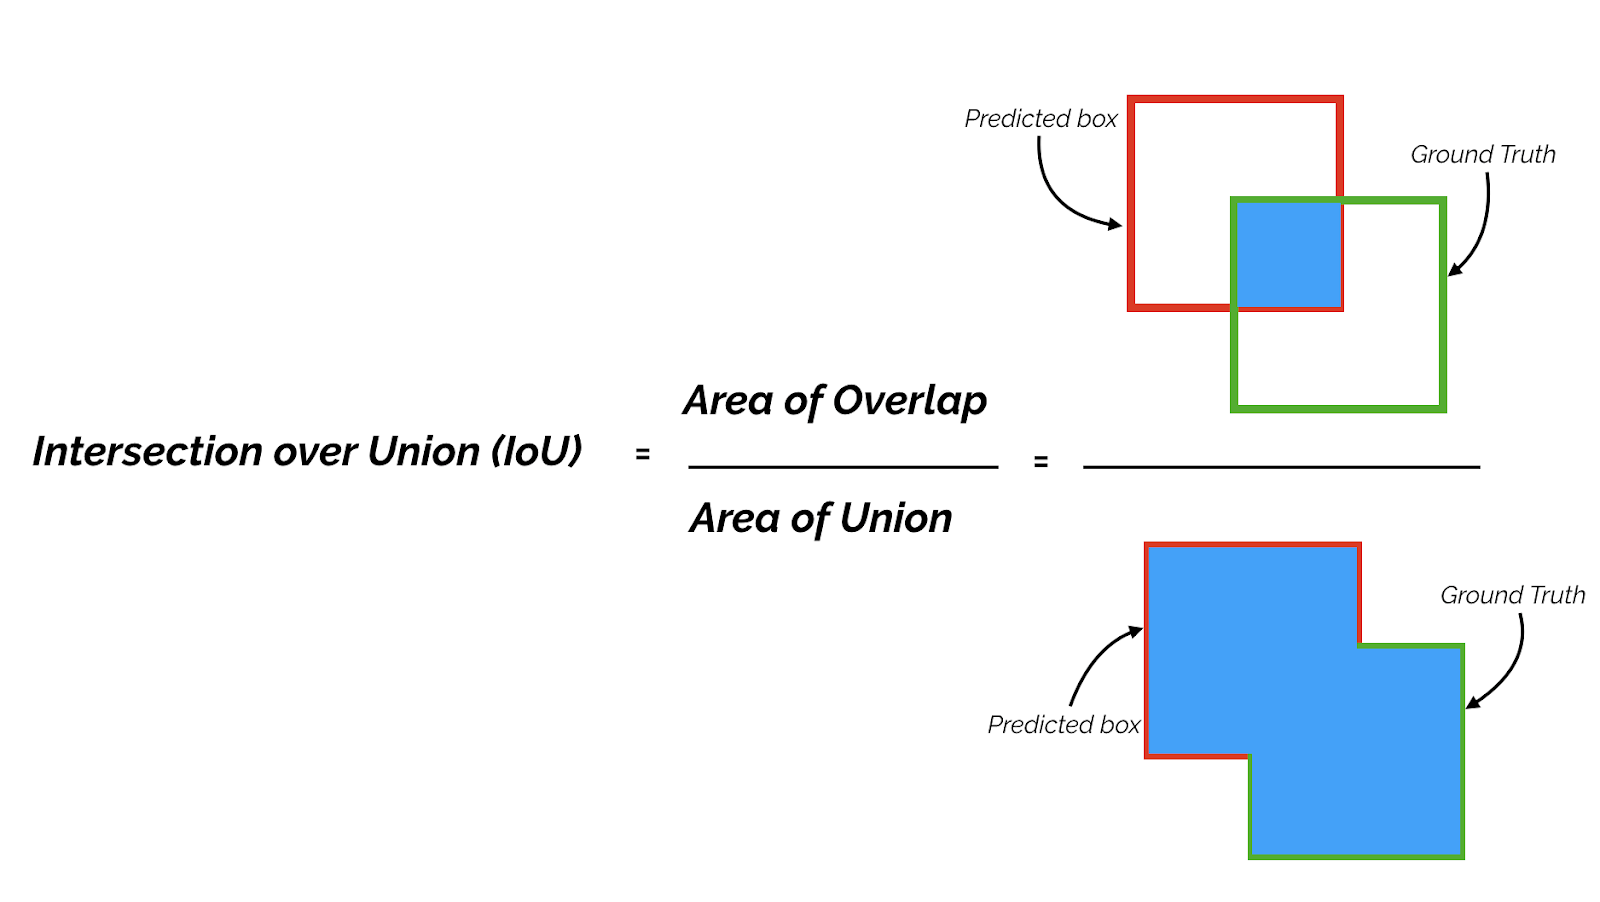
\includegraphics[width=0.65\textwidth]{img/chapters/resultados/metricas/iou.png}
\caption{\label{fig:iou}Área de superposición IoU entre los cuadros delimitadores}
\end{figure}

\subsubsection{TP, TN, FP y FN}
\label{subsubsec:tp+tn+fp+fn}

Otros parámetros básicos en las métricas de calidad que conforman la matriz de confusión \cite{confusion-matrix} son:

\begin{itemize}
    \item \textbf{\gls{tp}}: Número de predicciones donde el clasificador predice correctamente la clase positiva como positiva. \gls{iou} $\geqslant$ \textit{threshold}
    \item \textbf{\gls{tn}}: Número de predicciones donde el clasificador predice correctamente la clase negativa como negativa. No se utiliza en el cálculo de métricas.
    \item \textbf{\gls{fp}}: Número de predicciones donde el clasificador predice incorrectamente la clase negativa como positiva. \gls{iou} <\ \textit{threshold}
    \item \textbf{\gls{fn}}: Número de predicciones donde el clasificador predice incorrectamente la clase positiva como negativa.
\end{itemize}

Típicamente el \textit{threshold} toma valores del 50\%, 75\% o 95\%.

\begin{figure}[ht]
\centering
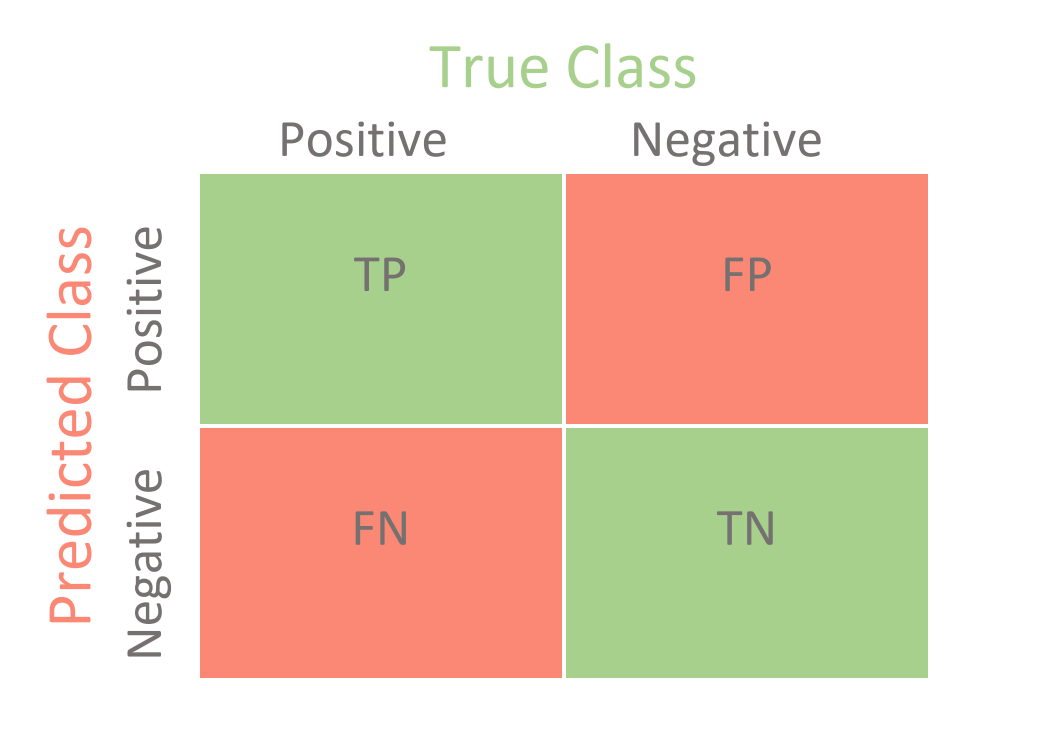
\includegraphics[width=0.45\textwidth]{img/chapters/resultados/metricas/confusion-matrix.png}
\caption{\label{fig:confusion-matrix}Matriz de confusión}
\end{figure}

\subsubsection{Precisión}
\label{subsubsec:precision}

La precisión es la capacidad de un modelo para identificar solo los objetos relevantes. Es el porcentaje de predicciones positivas correctas y viene dado por la siguiente expresión \ref{eq:precision}:

\begin{equation}
\label{eq:precision}
\text{P} = \frac{\text{TP}}{\text{TP}+\text{FP}}=\frac{\text{TP}}{\text{all detections}}
\end{equation}

\subsubsection{Exhaustividad}
\label{subsubsec:exhaustividad}

La exhaustividad es la capacidad de un modelo para encontrar todos los casos relevantes (todos los cuadros delimitadores de verdad del terreno). Es el porcentaje de verdadero positivo detectado entre todas las verdades fundamentales relevantes y viene dado por la siguiente expresión:

\begin{equation}
\label{eq:exhaustividad}
\text{R} = \frac{\text{TP}}{\text{TP}+\text{FN}}=\frac{\text{TP}}{\text{all ground truths}}
\end{equation}

\subsubsection{Valor-F}
\label{subsubsec:valor-f}

 El Valor-F se trata de una medida estadística de precisión muy utilizado en las pruebas test de algoritmos. Es la media armónica que combina los valores de la precisión y la exhaustividad. Viene dado por la expresión \ref{eq:valor-f}:

\begin{equation}
\label{eq:valor-f}
\text{F} = \frac{2 \cdotp \text{P} \cdotp \text{R}}{\text{P}+\text{R}}
\end{equation}

\textcolor{red}{Poner un ejemplo sencillo para que se entienda}

\subsubsection{Precisión media}
\label{subsubsec:averageprecision}

La precisión media es el valor medio de 11 puntos en la curva P-R para cada posible umbral (cada probabilidad de detección) para la misma clase (Precisión-Exhaustividad). En la ecuación \ref{eq:ap} se muestra el cálculo de la precisión media:

\begin{equation}
\label{eq:ap}
\text{AP}=\frac{1}{11} \sum_{r\in \left \{ 0, 0.1, ...,1 \right \}}\rho_{\text{interp}\left ( r \right )}
\end{equation}

con

$$\rho_{\text{interp}} = \max_{\tilde{r}:\tilde{r} \geq r} \rho\left ( \tilde{r} \right )$$

donde $\rho\left ( \tilde{r} \right )$ es la precisión medida en la exhaustividad $\tilde{r}$

Por otro lado, el \gls{map} es la media de los \gls{ap} de todas las categorías de objetos. El \gls{map} se representa mediante la siguiente ecuación:

\begin{equation}
\label{eq:map}
\text{mAP} = \frac{1}{N} \sum_{i=1}^{N} \text{AP}_{1}
\end{equation}

\subsection{Estrategia y metodología de experimentación}
\label{subsec:estrategia-metodologia}

\subsubsection{Entrenamiento con Open Image Dataset v4}
\label{subsubsec:train-openimagesv4}

\textcolor{red}{Aquí explicar como he entrenado una red neuronal con otro dataset a partir del repositorio \cite{OIDv4_ToolKit}}

\textcolor{red}{Explicar que se ha tomado 1500 imágenes de entrenamiento de las clases: person, handbag, backpack, suitcase y 300 imágenes de validación.}

\vspace{0.5cm}
\begin{lstlisting}[language=iPython,caption=Descarga dataset Open Images Dataset v4,captionpos=b,label={lst:download-oidv4}]
# Clonar el repositorio de Github
git clone https://github.com/theAIGuysCode/OIDv4_ToolKit.git
cd OIDv4_ToolKit

# Instalacion de las librerias y dependendencias
pip install -r requirements.txt

# Descarga de las imagenes de entrenamiento con un limite de 1500
python main.py downloader --classes Person Handbag Backpack Suitcase --type_csv train --limit 1500 --multiclasses 1

# Descarga de las imagenes de validacion con un limite de 300
python main.py downloader --classes Person Handbag Backpack Suitcase --type_csv validation --limit 300 --multiclasses 1

# Convertir etiquetas al formato de Darknet
python convert_annotations.py

\end{lstlisting}

\begin{figure}[ht]
\centering
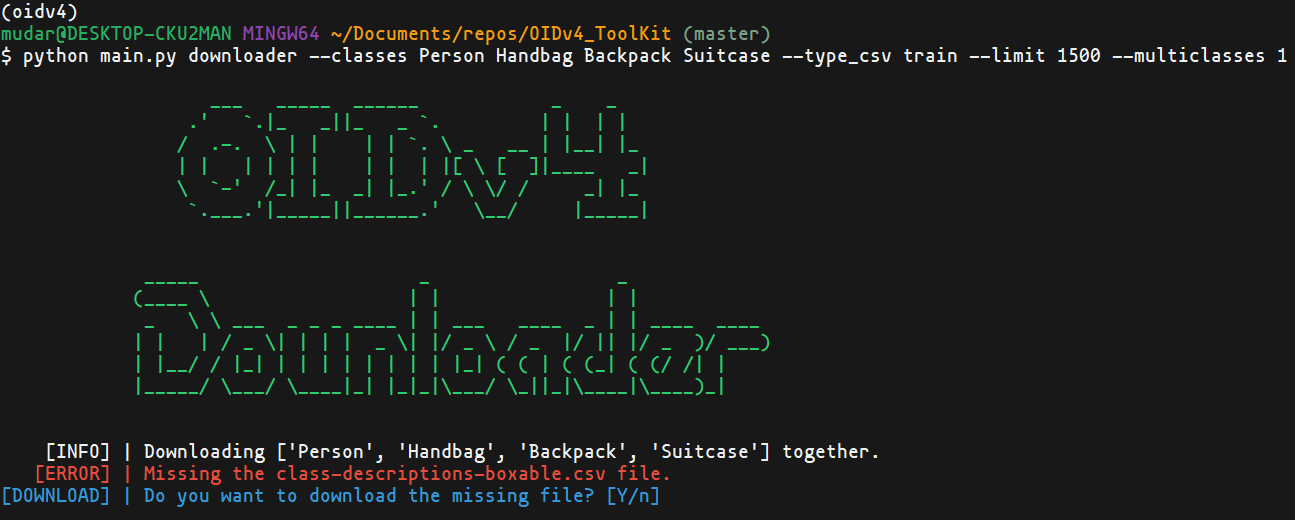
\includegraphics[width=0.3\textwidth]{img/chapters/resultados/datasets/download-oidv4.png}
\caption{\label{fig:download-oidv4}Descarga del dataset Open Images Dataset v4}
\end{figure}

\begin{figure}[ht]
\centering
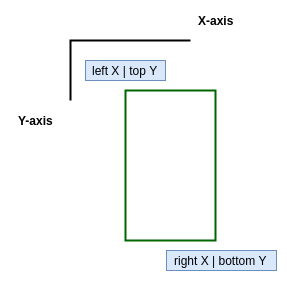
\includegraphics[width=0.3\textwidth]{img/chapters/resultados/datasets/bbox-oidv4.png}
\caption{\label{fig:bbox-oidv4}Estructura de las etiquetas de Open Images Dataset v4}
\end{figure}

La estructura que siguen las etiquetas del dataset de Open Images Dataset v4 es la siguiente:

\texttt{nombre de la clase x left top y x right bottom y}

\subsubsection{Métricas de calidad en Open Image Dataset v4}
\label{subsubsec:metricas-calidad-openimagesv4}

Tras entrenar YOLOv4 con el dataset personalizado que se ha explicado en el apartado anterior \ref{subsubsec:train-openimagesv4} se va a evaluar las métricas de calidad. Gracias al framework Darknet \cite{darknet13} es fácil poder evaluar las métricas aplicando el siguiente comando en el terminal:

\vspace{0.5cm}
\begin{lstlisting}[language=iPython,caption=Evaluación métricas de calidad del dataset utilizado para el entrenamiento de la red neuronal de detección de objetos,captionpos=b,label={lst:darknet-map}]
# Evaluacion de metricas de interes
./darknet detector train data/obj.data cfg/yolov4-obj.cfg yolov4.conv.137 -dont_show -map
\end{lstlisting}

\begin{figure}[ht]
\centering
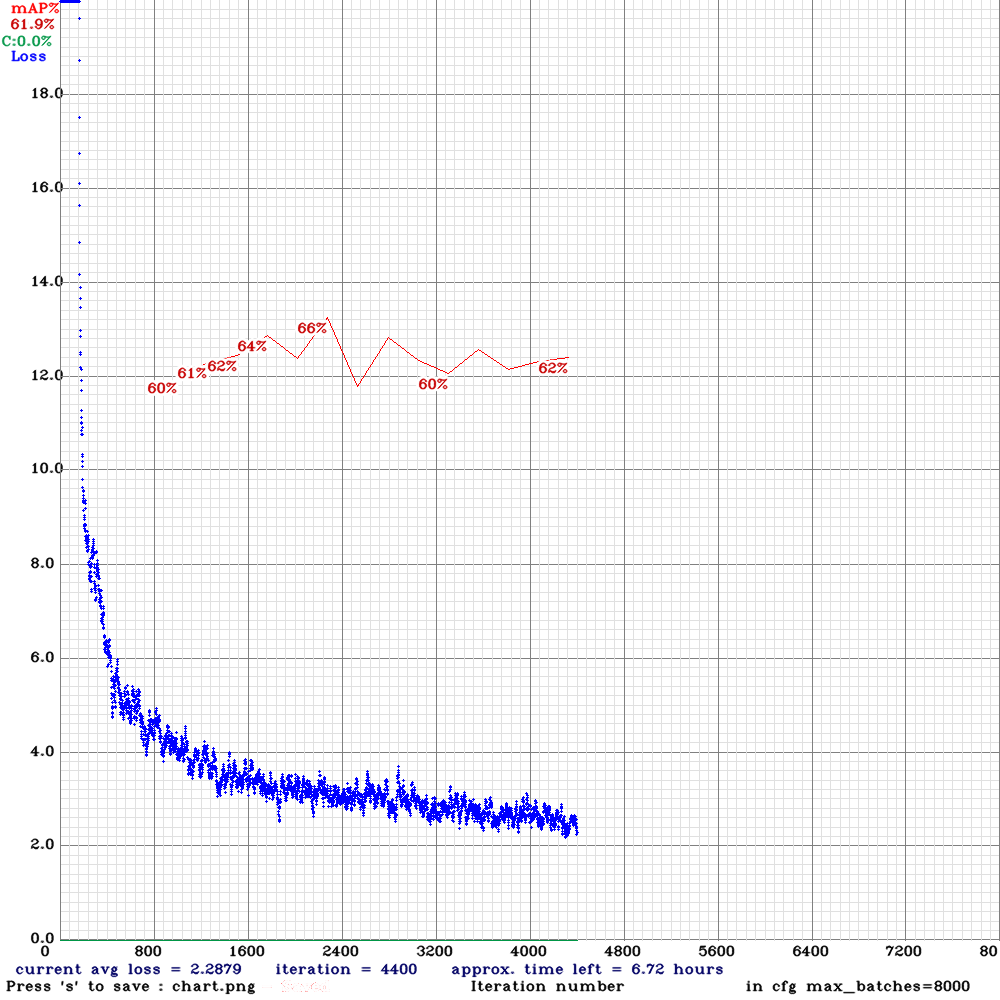
\includegraphics[width=0.3\textwidth]{img/chapters/resultados/metricas/chart_train.png}
\caption{\label{fig:chart-train}Evolución del mAP y pérdidas a lo largo de las interacciones durante el entrenamiento de la red neuronal con el dataset de OIDv4}
\end{figure}

\begin{figure}[ht]
\centering
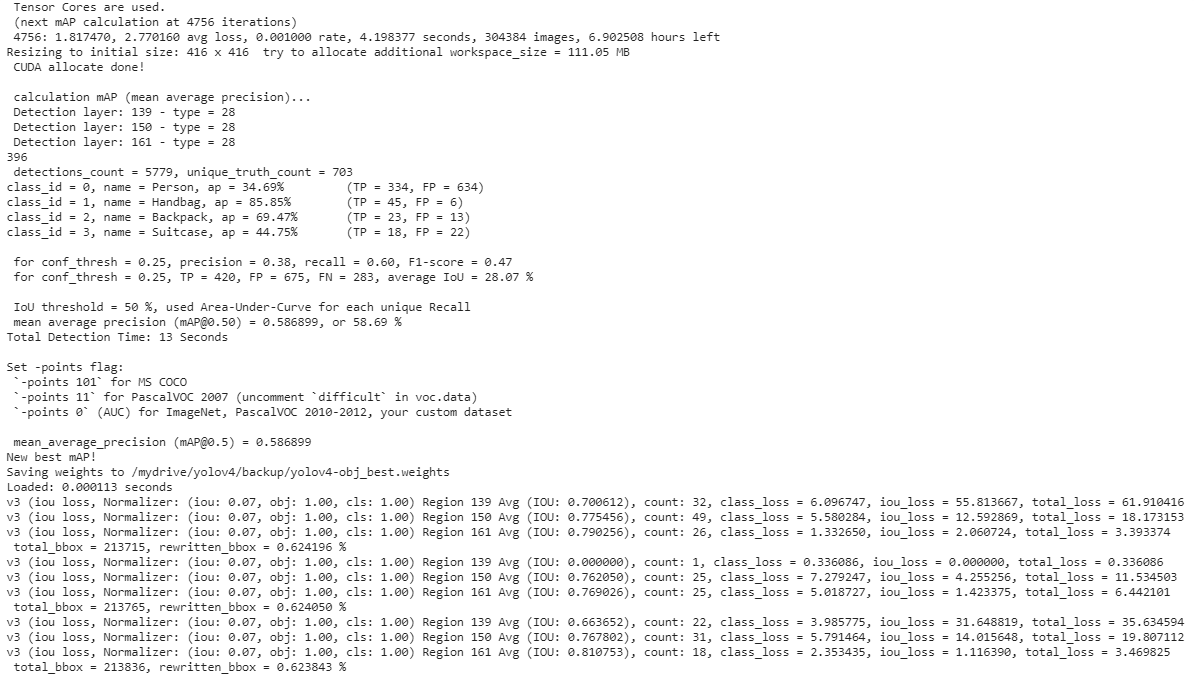
\includegraphics[width=0.3\textwidth]{img/chapters/resultados/metricas/metrics-during-training.png}
\caption{\label{fig:metrics-during-train}Métricas durante el entrenamiento de la red neuronal con el dataset de OIDv4}
\end{figure}

En la tabla \ref{tab:metricas-test1_1}, \ref{tab:metricas-test1_2}, \ref{tab:metricas-test1_3} y \ref{tab:metricas-test1_4} se reflejan las métricas más relevantes cada 1000 iteraciones del entrenamiento de la red neuronal.

\begin{table}[ht]
\centering
\caption{Métricas de calidad en el primer entrenamiento con OIDv4 [1]}
\label{tab:metricas-test1_1}
\begin{tabular}{lcccc}
\hline
\textbf{Iterations} & \textbf{\begin{tabular}[c]{@{}c@{}}AP person\\ (\%)\end{tabular}} & \textbf{\begin{tabular}[c]{@{}c@{}}AP handbag\\ (\%)\end{tabular}} & \textbf{\begin{tabular}[c]{@{}c@{}}AP backpack\\ (\%)\end{tabular}} & \textbf{\begin{tabular}[c]{@{}c@{}}AP suitcase\\ (\%)\end{tabular}} \\ \hline
1.000               & 31,26                                                             & 85,45                                                              & 67,99                                                               & 42,15                                                               \\
\textbf{2.000}      & \textbf{43,96}                                                    & \textbf{92,39}                                                     & \textbf{63,88}                                                      & \textbf{64,79}                                                      \\
3.000               & 36,16                                                             & 90,10                                                              & 67,88                                                               & 53,33                                                               \\
4.000               & 35,56                                                             & 91,99                                                              & 64,61                                                               & 57,74                                                               \\
5.000               & 34,21                                                             & 87,35                                                              & 68,73                                                               & 48,77                                                               \\
6.000               & 36,74                                                             & 89,48                                                              & 65,83                                                               & 49,09                                                               \\
7.000               & 34,76                                                             & 88,94                                                              & 68,20                                                               & 51,24                                                               \\
8.000               & 38,30                                                             & 87,69                                                              & 72,00                                                               & 58,89                                                               \\ \hline
\end{tabular}
\end{table}

\newpage

\begin{table}[ht]
\centering
\caption{Métricas de calidad en el primer entrenamiento con OIDv4 [2]}
\label{tab:metricas-test1_2}
\begin{tabular}{lcccc}
\hline
\textbf{Iterations} & \textbf{TP person} & \textbf{TP handbag} & \textbf{TP backpack} & \textbf{TP suitcase} \\ \hline
1.000               & 249                & 52                  & 19                   & 16                   \\
\textbf{2.000}      & \textbf{338}       & \textbf{54}         & \textbf{19}          & \textbf{19}          \\
3.000               & 324                & 54                  & 21                   & 18                   \\
4.000               & 329                & 54                  & 20                   & 20                   \\
5.000               & 313                & 50                  & 23                   & 16                   \\
6.000               & 323                & 52                  & 20                   & 13                   \\
7.000               & 288                & 53                  & 19                   & 18                   \\
8.000               & 308                & 49                  & 21                   & 19                   \\ \hline
\end{tabular}
\end{table}

\begin{table}[ht]
\centering
\caption{Métricas de calidad en el primer entrenamiento con OIDv4 [3]}
\label{tab:metricas-test1_3}
\begin{tabular}{lcccc}
\hline
\textbf{Iterations} & \textbf{FP person} & \textbf{FP handbag} & \textbf{FP backpack} & \textbf{FP suitcase} \\ \hline
1.000               & 416                & 20                  & 11                   & 42                   \\
\textbf{2.000}      & \textbf{489}       & \textbf{15}         & \textbf{16}          & \textbf{7}           \\
3.000               & 479                & 22                  & 18                   & 36                   \\
4.000               & 521                & 10                  & 20                   & 19                   \\
5.000               & 474                & 14                  & 19                   & 22                   \\
6.000               & 446                & 7                   & 14                   & 13                   \\
7.000               & 391                & 19                  & 13                   & 16                   \\
8.000               & 412                & 11                  & 16                   & 17                   \\ \hline
\end{tabular}
\end{table}

\begin{table}[ht!]
\centering
\caption{Métricas de calidad en el primer entrenamiento con OIDv4 [4]}
\label{tab:metricas-test1_4}
\begin{tabular}{lcccccccc}
\hline
\textbf{Iterations} & \textbf{TP}  & \textbf{FP}  & \textbf{FN}  & \textbf{\begin{tabular}[c]{@{}c@{}}Precision\\ (\%)\end{tabular}} & \textbf{\begin{tabular}[c]{@{}c@{}}Recall\\ (\%)\end{tabular}} & \textbf{\begin{tabular}[c]{@{}c@{}}F-score\\ (\%)\end{tabular}} & \textbf{\begin{tabular}[c]{@{}c@{}}Average IoU\\ (\%)\end{tabular}} & \textbf{\begin{tabular}[c]{@{}c@{}}mAP @ 0.5\\ (\%)\end{tabular}} \\ \hline
1.000               & 336          & 489          & 367          & 40,73                                                             & 47,80                                                          & 43,98                                                           & 29,36                                                               & 56,71                                                             \\
\textbf{2.000}      & \textbf{430} & \textbf{527} & \textbf{273} & \textbf{44,93}                                                    & \textbf{61,17}                                                 & \textbf{51,81}                                                  & \textbf{34,13}                                                      & \textbf{66,25}                                                    \\
3.000               & 417          & 555          & 286          & 42,90                                                             & 59,32                                                          & 49,79                                                           & 32,29                                                               & 61,87                                                             \\
4.000               & 423          & 570          & 280          & 42,60                                                             & 60,17                                                          & 49,88                                                           & 33,30                                                               & 62,47                                                             \\
5.000               & 402          & 529          & 301          & 43,18                                                             & 57,18                                                          & 49,20                                                           & 32,53                                                               & 59,77                                                             \\
6.000               & 408          & 480          & 295          & 45,95                                                             & 58,04                                                          & 51,29                                                           & 36,76                                                               & 60,28                                                             \\
7.000               & 378          & 439          & 325          & 46,27                                                             & 53,77                                                          & 49,74                                                           & 36,90                                                               & 60,78                                                             \\
8.000               & 397          & 456          & 306          & 46,54                                                             & 56,47                                                          & 51,03                                                           & 37,69                                                               & 64,22                                                             \\ \hline
\end{tabular}
\end{table}

\newpage

\textcolor{red}{Aquí explicar porque en función de las métricas obtenidas no es un buen modelo y se debe de reentrenar la red. El \gls{iou} sale muy bajo <\ 50\%, por tanto salen muchos FP}

\begin{table}[ht]
\centering
\caption{Métricas de calidad en el segundo entrenamiento con OIDv4 [1]}
\label{tab:metricas-test2_1}
\begin{tabular}{lcccccc}
\hline
\textbf{Iterations} & \textbf{\begin{tabular}[c]{@{}c@{}}AP person\\ (\%)\end{tabular}} & \textbf{\begin{tabular}[c]{@{}c@{}}AP bags\\ (\%)\end{tabular}} & \textbf{TP person} & \textbf{TP bags} & \textbf{FP person} & \textbf{FP bags} \\ \hline
1.000               & 30,81                                                             & 21,61                                                           & 5.216              & 231               & 9.220              & 579              \\
2.000               & 38,38                                                             & 53,59                                                           & 6.542              & 362               & 11.789             & 354              \\
3.000               & 33,51                                                             & 68,56                                                           & 7.232              & 419               & 18.887             & 411              \\
4.000               & 41,31                                                             & 77,12                                                           & 7.105              & 427               & 11.397             & 222              \\
5.000               & 38,86                                                             & 75,78                                                           & 6.586              & 444               & 11.735             & 398              \\
6.000               & 36,29                                                             & 66,49                                                           & 6.556              & 426               & 12.506             & 537              \\
7.000               & 39,94                                                             & 67,78                                                           & 6.246              & 418               & 9.744              & 523              \\
8.000               & 31,69                                                             & 69,07                                                           & 6.082              & 417               & 13.353             & 422              \\
9.000               & 43,34                                                             & 78,37                                                           & 6.773              & 451               & 9.846              & 373              \\
\textbf{10.000}     & \textbf{43,40}                                                    & \textbf{78,53}                                                  & \textbf{6.174}     & \textbf{426}      & \textbf{7.149}     & \textbf{217}     \\
11.000              & 38,81                                                             & 76,60                                                           & 7.166              & 446               & 12.162             & 387              \\
12.000              & 41,72                                                             & 78,10                                                           & 6.926              & 444               & 10.387             & 289              \\
13.000              & 39,48                                                             & 74,67                                                           & 6.575              & 406               & 9.850              & 238              \\
14.000              & 41,85                                                             & 73,69                                                           & 6.844              & 432               & 10.092             & 385              \\
15.000              & 40,19                                                             & 75,37                                                           & 6.915              & 423               & 11.426             & 252              \\
16.000              & 41,26                                                             & 75,17                                                           & 6.661              & 423               & 9.330              & 219              \\
17.000              & 42,13                                                             & 78,77                                                           & 6.991              & 433               & 9.924              & 242              \\
18.000              & 40,97                                                             & 75,45                                                           & 6.871              & 432               & 10.243             & 300              \\
19.000              & 39,01                                                             & 73,23                                                           & 6.822              & 428               & 10.791             & 333              \\
20.000              & 41,37                                                             & 78,38                                                           & 7.011              & 432               & 10.103             & 232              \\ \hline
\end{tabular}
\end{table}

\begin{table}[ht!]
\centering
\caption{Métricas de calidad en el segundo entrenamiento con OIDv4 [2]}
\label{tab:metricas-test2_2}
\begin{tabular}{lcccccccc}
\hline
\textbf{Iterations} & \textbf{TP}    & \textbf{FP}    & \textbf{FN}    & \textbf{\begin{tabular}[c]{@{}c@{}}Precision\\ (\%)\end{tabular}} & \textbf{\begin{tabular}[c]{@{}c@{}}Recall\\ (\%)\end{tabular}} & \textbf{\begin{tabular}[c]{@{}c@{}}F-score\\ (\%)\end{tabular}} & \textbf{\begin{tabular}[c]{@{}c@{}}Average\\ IoU (\%)\end{tabular}} & \textbf{\begin{tabular}[c]{@{}c@{}}mAP @ 0.5\\ (\%)\end{tabular}} \\ \hline
1.000               & 5.447          & 9.799          & 6.379          & 35,73                                                             & 46,06                                                          & 40,24                                                           & 25,72                                                               & 26,21                                                             \\
2.000               & 6.904          & 12.143         & 4.922          & 36,25                                                             & 58,38                                                          & 44,73                                                           & 27,30                                                               & 45,98                                                             \\
3.000               & 7.651          & 19.298         & 4.175          & 28,39                                                             & 64,70                                                          & 39,46                                                           & 21,66                                                               & 51,04                                                             \\
4.000               & 7.532          & 11.619         & 4.294          & 39,33                                                             & 63,69                                                          & 48,63                                                           & 30,90                                                               & 59,22                                                             \\
5.000               & 7.030          & 12.133         & 4.796          & 36,69                                                             & 59,45                                                          & 45,37                                                           & 28,28                                                               & 57,32                                                             \\
6.000               & 6.982          & 13.043         & 4.844          & 34,87                                                             & 59,04                                                          & 43,84                                                           & 27,23                                                               & 51,39                                                             \\
7.000               & 6.664          & 10.267         & 5.162          & 39,36                                                             & 56,35                                                          & 46,35                                                           & 30,96                                                               & 53,86                                                             \\
8.000               & 6.499          & 13.775         & 5.327          & 32,06                                                             & 54,96                                                          & 40,49                                                           & 24,96                                                               & 50,38                                                             \\
9.000               & 7.224          & 10.219         & 4.602          & 41,41                                                             & 61,09                                                          & 49,36                                                           & 32,95                                                               & 60,85                                                             \\
\textbf{10.000}     & \textbf{6.600} & \textbf{7.366} & \textbf{5.226} & \textbf{47,26}                                                    & \textbf{55,81}                                                 & \textbf{51,18}                                                  & \textbf{37,83}                                                      & \textbf{60,97}                                                    \\
11.000              & 7.612          & 12.549         & 4.214          & 37,76                                                             & 64,37                                                          & 47,59                                                           & 30,20                                                               & 57,70                                                             \\
12.000              & 7.370          & 10.676         & 4.456          & 40,84                                                             & 62,32                                                          & 49,34                                                           & 32,34                                                               & 59,91                                                             \\
13.000              & 6.981          & 10.088         & 4.845          & 40,90                                                             & 59,03                                                          & 48,32                                                           & 32,83                                                               & 57,07                                                             \\
14.000              & 7.276          & 10.477         & 4.550          & 40,98                                                             & 61,53                                                          & 49,20                                                           & 32,61                                                               & 57,77                                                             \\
15.000              & 7.338          & 11.678         & 4.488          & 38,59                                                             & 62,05                                                          & 47,58                                                           & 30,53                                                               & 57,78                                                             \\
16.000              & 7.084          & 9.549          & 4.742          & 42,59                                                             & 59,90                                                          & 49,78                                                           & 33,87                                                               & 58,22                                                             \\
17.000              & 7.424          & 10.166         & 4.402          & 42,21                                                             & 62,78                                                          & 50,48                                                           & 34,53                                                               & 60,45                                                             \\
18.000              & 7.303          & 10.543         & 4.523          & 40,92                                                             & 61,75                                                          & 49,22                                                           & 33,11                                                               & 58,21                                                             \\
19.000              & 7.250          & 11.124         & 4.576          & 39,46                                                             & 61,31                                                          & 48,01                                                           & 31,90                                                               & 56,12                                                             \\
20.000              & 7.443          & 10.335         & 4.383          & 41,87                                                             & 62,94                                                          & 50,28                                                           & 34,35                                                               & 59,93                                                             \\ \hline
\end{tabular}
\end{table}

\newpage

\subsubsection{Métricas de calidad en MS COCO 2017 Dataset}
\label{subsubsec:metricas-calidad-coco}

\begin{table}[ht]
\centering
\caption{Comparativa métricas de calidad entre los test en OIDv4 y MS COCO 2017 [1]}
\label{tab:comparativa-metricas1}
\begin{tabular}{lccc}
\hline
\textbf{Dataset}                   & \textbf{TP}          & \textbf{FP}          & \textbf{FN}          \\ \hline
\textbf{MS COCO 2017}              & \textbf{22.730}      & \textbf{10.889}      & \textbf{13.027}      \\
OIDv4 test 1                       & 430                  & 527                  & 273                \\
OIDv4 test 2                       & 6.600                & 7.366                & 5.226                \\ \hline
\end{tabular}
\end{table}

\begin{table}[ht]
\centering
\caption{Comparativa métricas de calidad entre los dos test en OIDv4 y MS COCO 2017 [2]}
\label{tab:comparativa-metricas2}
\begin{tabular}{cccccc}
\hline
\rowcolor[HTML]{FFFFFF} 
\textbf{Dataset}             & \textbf{\begin{tabular}[c]{@{}c@{}}Precision\\ (\%)\end{tabular}} & \textbf{\begin{tabular}[c]{@{}c@{}}Recall\\ (\%)\end{tabular}} & \textbf{\begin{tabular}[c]{@{}c@{}}F-score\\ (\%)\end{tabular}} & \textbf{\begin{tabular}[c]{@{}c@{}}average IoU\\ (\%)\end{tabular}} & \textbf{\begin{tabular}[c]{@{}c@{}}mAP @ 0.5\\ (\%)\end{tabular}} \\ \hline
\textbf{MS COCO 2017}        & \textbf{67,61}                                                    & \textbf{63,57}                                                 & \textbf{65,53}                                                  & \textbf{56.04}                                                      & \textbf{64.16}                                                    \\
OIDv4 test 1                 & 44,93                                                             & 61,17                                                          & 51,81                                                           & 34,13                                                               & 66,25                                                             \\
OIDv4 test 2                 & 47,26                                                             & 55,81                                                          & 51,18                                                           & 37,83                                                               & 60,97                                                             \\ \hline
\end{tabular}
\end{table}

\begin{table}[ht]
\centering
\caption{Métricas de calidad de MS COCO 2017 en las clases de interés}
\label{tab:metricas-clases-coco}
\begin{tabular}{lccc}
\hline
\textbf{Class} & \textbf{AP(\%)} & \textbf{TP} & \textbf{FP} \\ \hline
Person         & 79,53           & 7.923       & 3.168       \\
Backpack       & 44,10           & 172         & 156         \\
Handbag        & 29,83           & 158         & 215         \\
Suitcase       & 71,08           & 205         & 102         \\ \hline
\end{tabular}
\end{table}

\newpage

\begin{figure}[ht]
\centering
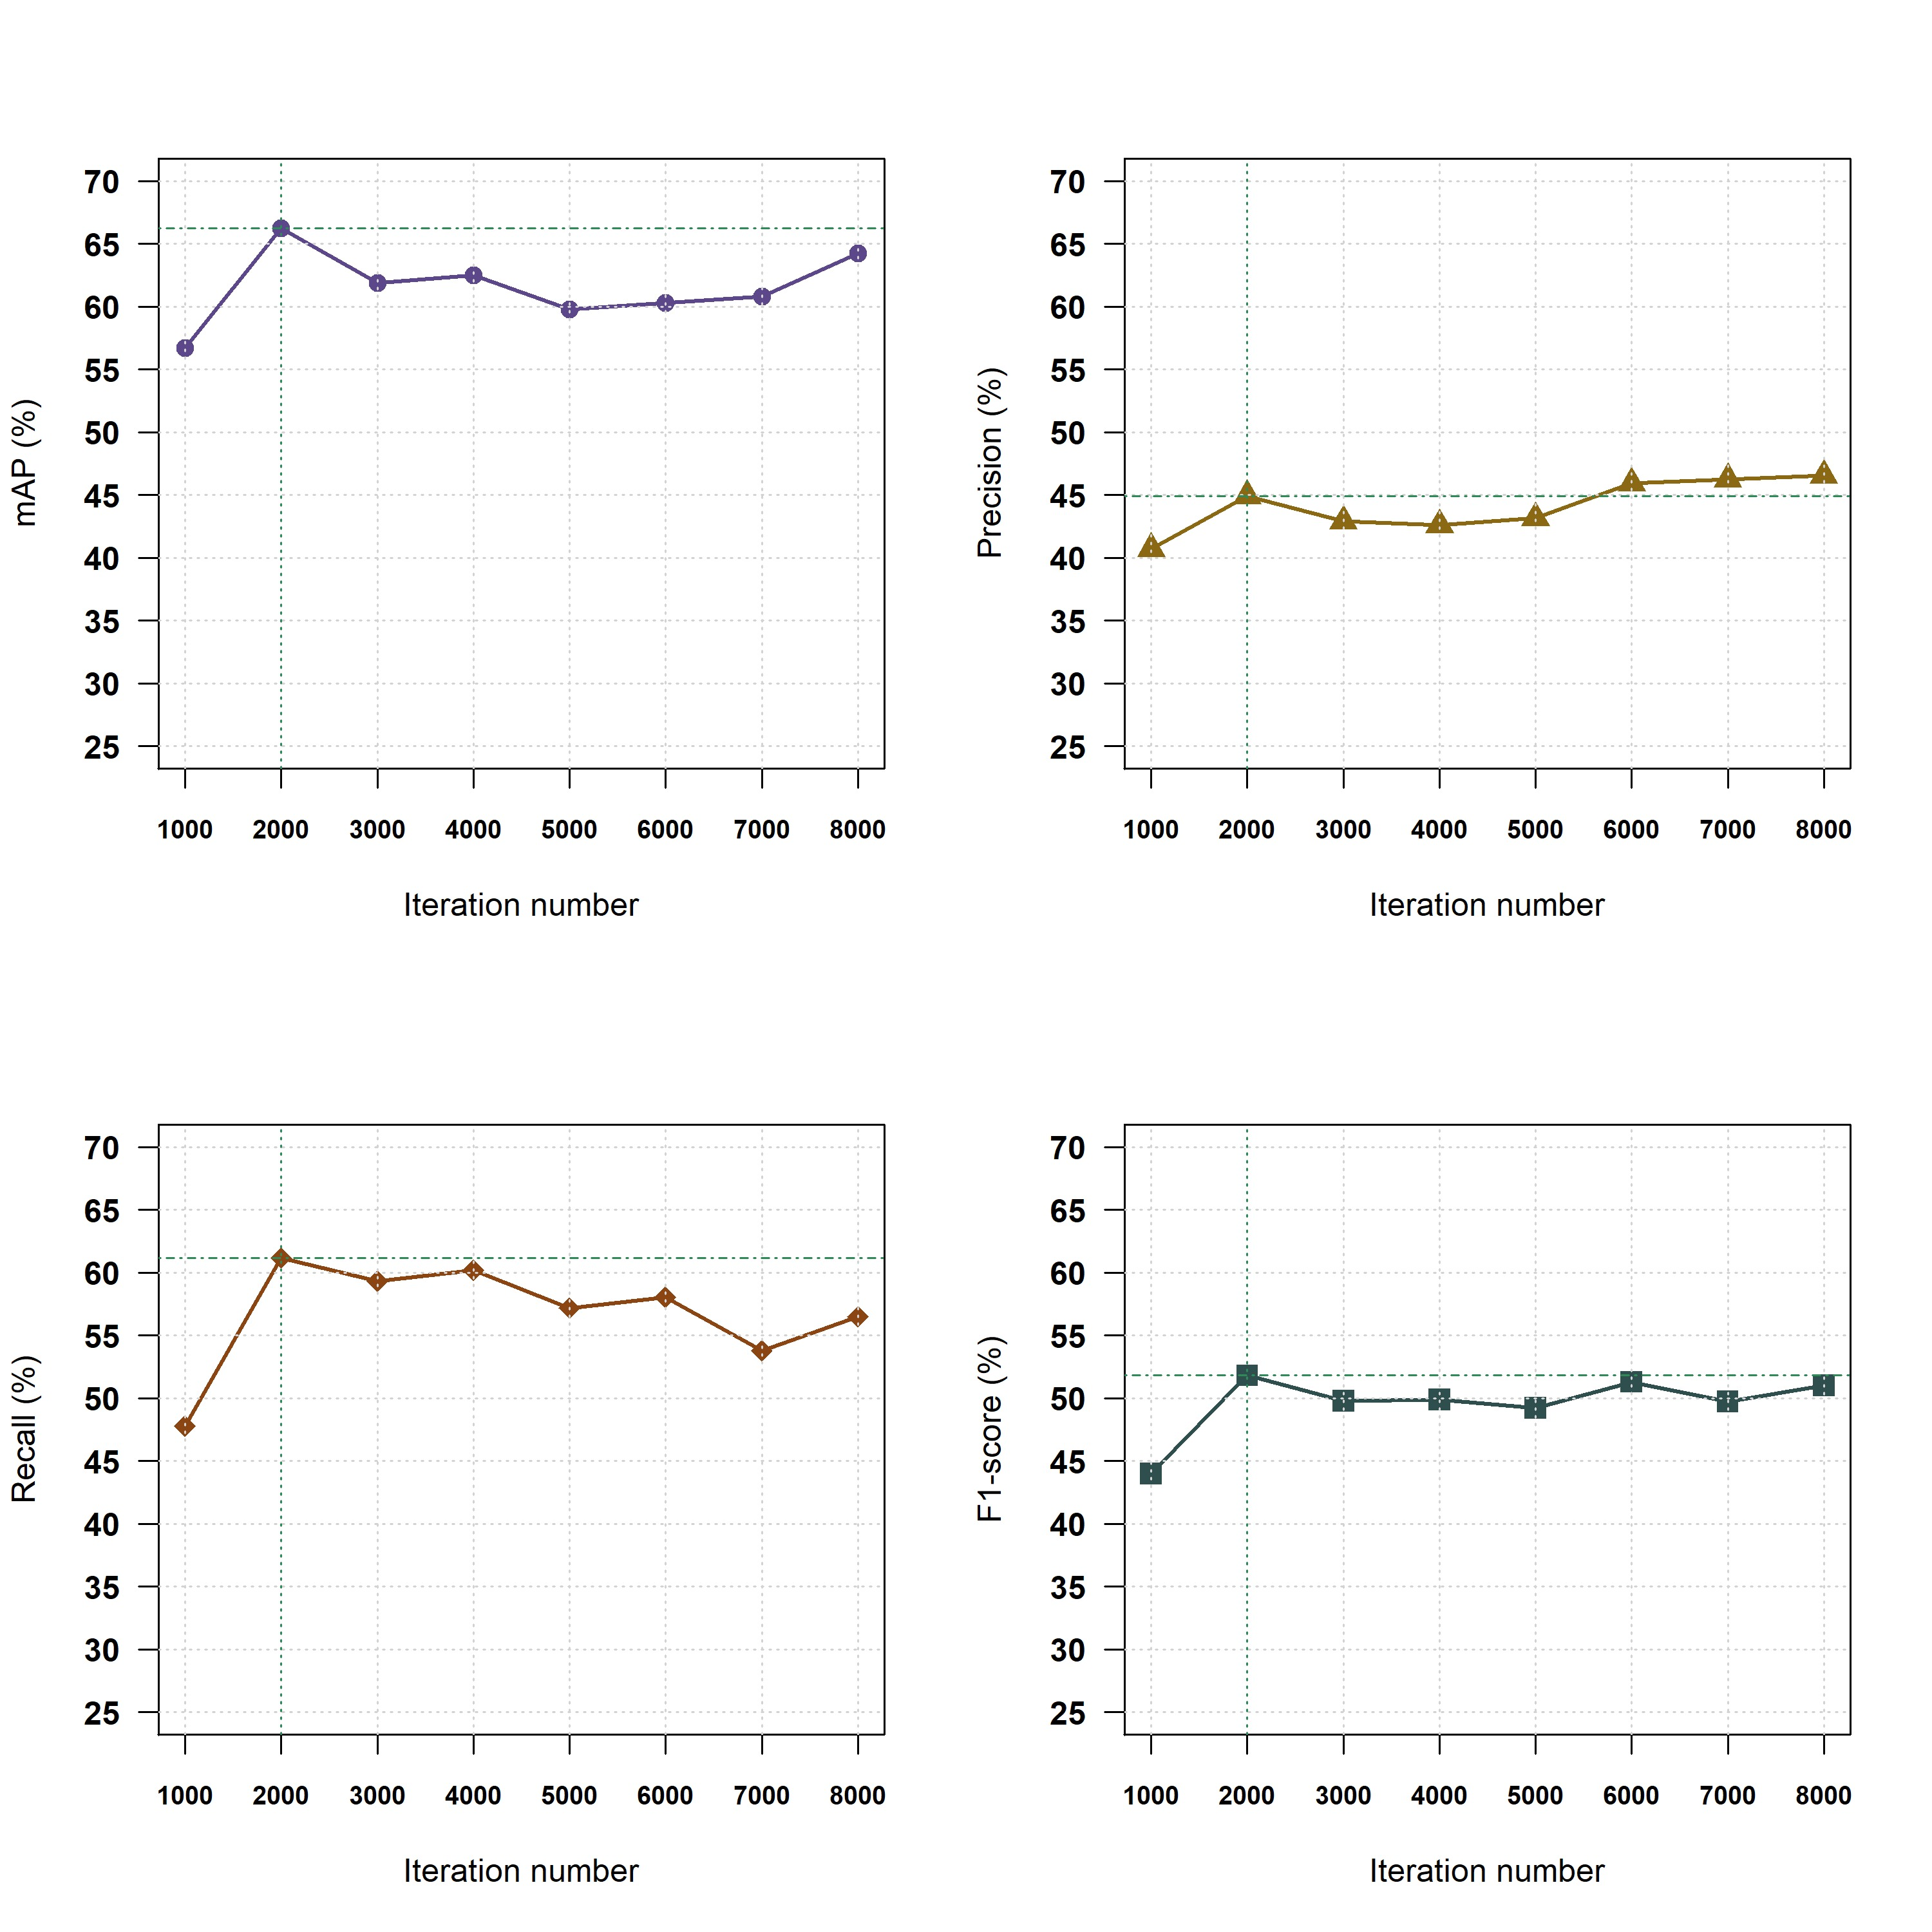
\includegraphics[width=1\textwidth]{img/chapters/resultados/metricas/metrics-train1.png}
\caption{\label{fig:metrics-train1}Resumen métricas primer entrenamiento de la red neuronal con el dataset de OIDv4}
\end{figure}

\newpage

\begin{figure}[ht]
\centering
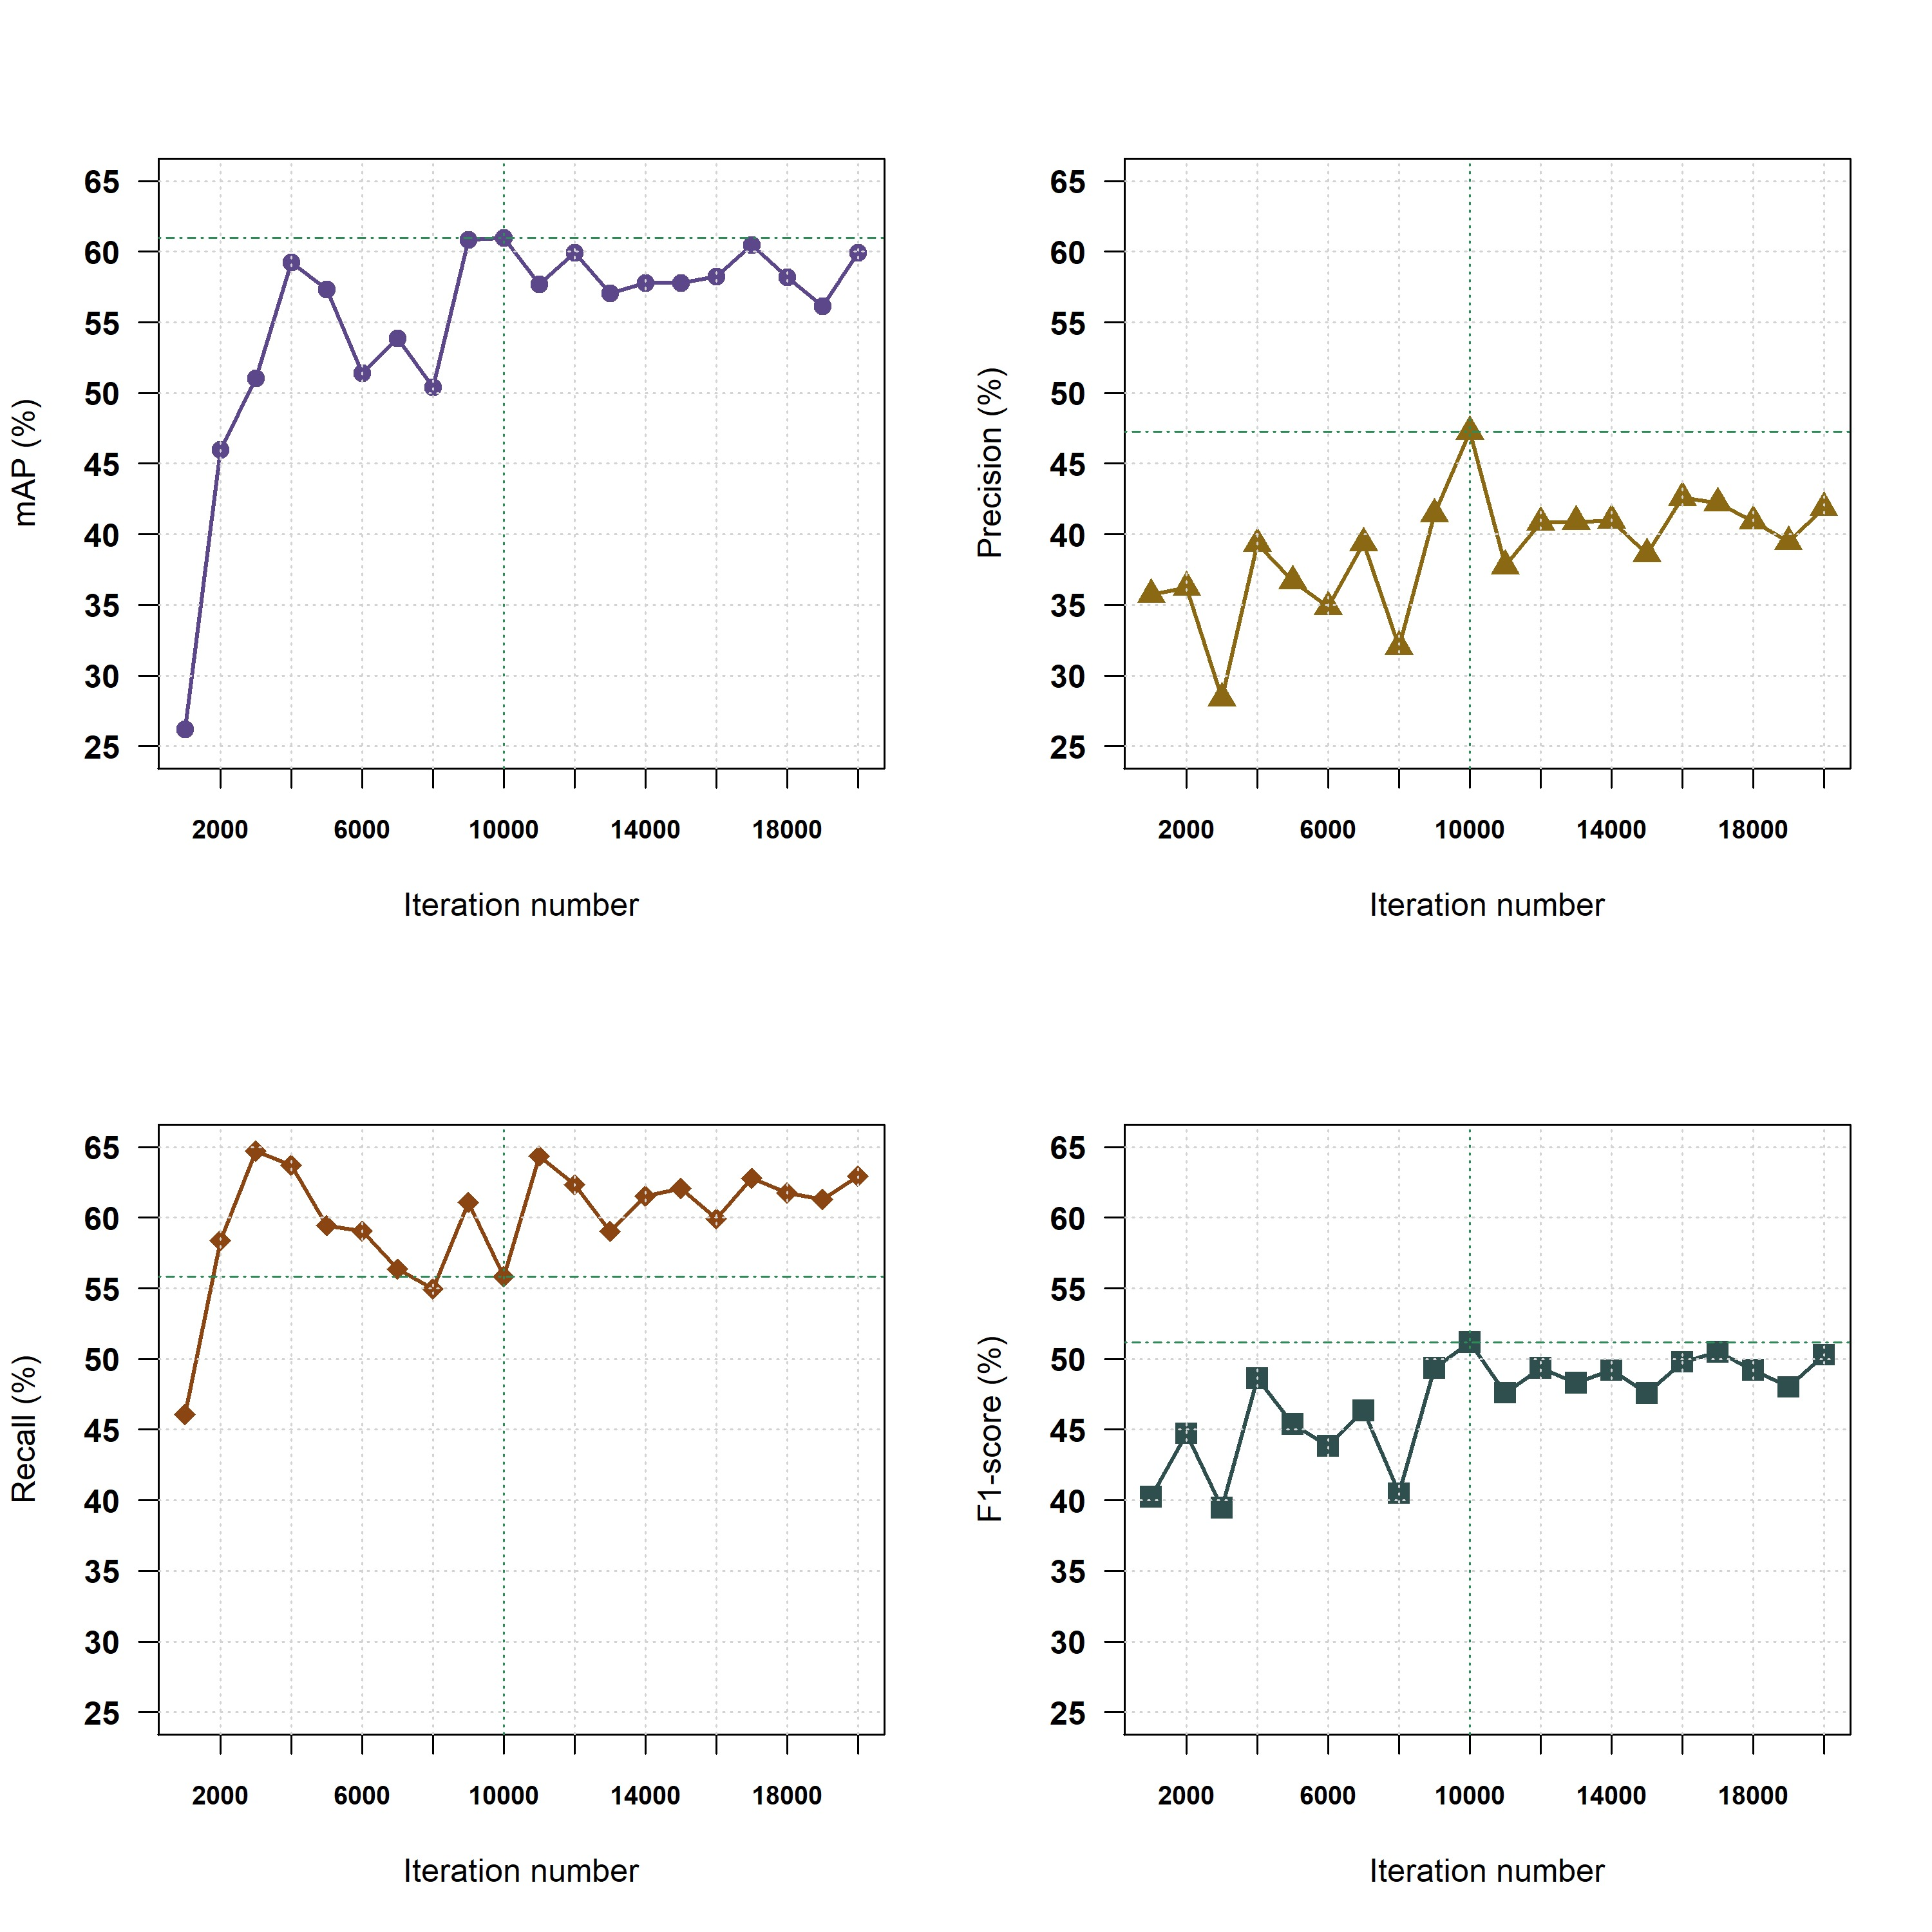
\includegraphics[width=1\textwidth]{img/chapters/resultados/metricas/metrics-train2.png}
\caption{\label{fig:metrics-train2}Resumen métricas segundo entrenamiento de la red neuronal con el dataset de OIDv4}
\end{figure}

\newpage

\section{Resultados experimentales}
\label{sec:resultados-experimentales}

Una vez elegido MS COCO 2017 como dataset de referencia para usar con YOLOv4, se va a ver los resultados obtenidos en distintos algoritmos.

\subsection{Resultados en detección de objetos con YOLOv4}
\label{subsec:resultados-yolov4-tf}

\textcolor{red}{Poner imágenes de las detecciones en los datasets empleados y explicar con detalle como influye distintos elementos como la distancia, iluminación, color, etc... en la detección de objetos}.

\url{https://old.photojoiner.net/}

\textcolor{red}{También hacer tablas durante un número determinado de frames donde, a modo de ejemplo se calcule las métricas más relevantes}.

\subsection{Resultados en tracking con DeepSORT}
\label{subsec:resultados-deepsort}

\textcolor{red}{Poner imágenes de las detecciones en los datasets empleados y explicar con detalle los problemas con los que nos podemos encontrar a la hora de hacer un seguimiento o \textit{tracking} de objetos y personas, se pierde el rastreo y se vuelve a asociar una nueva ID a ese individuo, también explicar que debido al \textit{threshold} que pongamos se pueden perder objetos, pero tampoco es conveniente bajarlo a más de X porque entonces se confunden objetos o se trackean varias veces}.

\subsection{Resultados en algoritmo de detección de objetos abandonados}
\label{subsec:resultados-abandon-algorithm}

\textcolor{red}{Poner imágenes de detecciones de objetos abandonados y explicar de manera visual como es posible que hayan problemas cuando se pierde el \textit{tracking} de un objeto o persona y se tiene que reasignar como nuevo ID y posteriormente tener que volver a hacer una asociación de persona-objeto y evaluar si se abandona o no dicho objeto}.

\textcolor{red}{Aquí meter un subsubapartado con métricas relevantes en la detección de objetos abandonados}.

\section{Conclusiones}
\label{sec:conclu-resultados}